% !TEX program = xelatex
\documentclass[oneside,master]{zjuthesis}
% 默认为单面模式,如需打印请把oneside换为twoside,博士请将master换为doctor
%==============================================================
%==============================================================

%自己需要增加什么 package 或修改什么设置的话,都放在这里吧。
\usepackage{enumerate}
\usepackage[perpage,symbol]{footmisc}
\setfnsymbol{wiley}
\usepackage{hypbmsec}
\usepackage{dsfont}
\usepackage{listings}
\usepackage{xcolor}

\newcommand{\tabincell}[2]{\begin{tabular}{@{}#1@{}}#2\end{tabular}}

%==============================================================
%==============================================================
\begin{document}

%==============================================================
%==============================================================
%这部分是论文封面、题名页需要的信息,请根据《研究生学位论文编写规则》自行修改

%论文分类号
  \renewcommand{\zjuclass}{TM888} 

%论文密级
  \renewcommand{\zjusecurity}{}
 
\renewcommand{\zjutitlec}{***********}%中文论文题目
\renewcommand{\zjutitlecb}{}%中文论文题目第二行,若无请留空
\renewcommand{\zjutitlecc}{}%中文论文题目第三行,若无请留空
\renewcommand{\zjutitlee}{***********}%英文论文题目
\renewcommand{\zjutitleeb}{}%英文论文题目第二行,若无请留空
\renewcommand{\zjutitleec}{}%英文论文题目第三行,若无请留空

%作者姓名
  \renewcommand{\zjuauthor}{袁淳} 

%作者学号
  \renewcommand{\zjuauthorid}{21935006}

%指导教师 
  \renewcommand{\zjumentor}{杨勋年}

%合作导师(如果有的话请取消注释)
  %\renewcommand{\zjumentorco}{}

%专业名称
  \renewcommand{\zjumajor}{应用数学}

%研究方向
  \renewcommand{\zjusubject}{物理模拟}

%所在学院
  \renewcommand{\zjuschool}{数学科学学院}

%提交日期
  \renewcommand{\zjuapprovaldate}{二〇一九年四月}

%答辩日期
  \renewcommand{\zjudefencedatec}{二〇一九年六月}
  \renewcommand{\zjudefencedatee}{June 2019}

%论文评阅人(格式:姓名 ~ 职称 ~ 单位)
  \renewcommand{\zjurevieweronec}{陈某某 ~ 教授 ~ XX大学}
  \renewcommand{\zjurevieweronee}{Moumou Chen ~Prof. ~XX University}

  \renewcommand{\zjureviewertwoc}{张某某 ~ 教授 ~ XX大学}
  \renewcommand{\zjureviewertwoe}{Moumou Zhang ~Prof. ~XX University}

  \renewcommand{\zjureviewerthreec}{李某某 ~ 教授 ~ XX大学}
  \renewcommand{\zjureviewerthreee}{Moumou Li ~Prof. ~XX University }

  \renewcommand{\zjureviewerfourc}{吴某某 ~ 教授 ~ XX大学}
  \renewcommand{\zjureviewerfoure}{Moumou Wu ~Prof. ~XX University}

  \renewcommand{\zjureviewerfivec}{杨某某 ~ 教授 ~ XX大学}
  \renewcommand{\zjureviewerfivee}{Moumou Yang ~Prof. ~XX University}

%答辩委员会(姓名\职称\单位)
  \renewcommand{\zjucommitteemainc}{郑某某 ~ 教授 ~ 浙江大学}
  \renewcommand{\zjucommitteemaine}{Moumou Zheng~ Prof. ~Zhejiang University}

  \renewcommand{\zjucommitteeonec}{郑某某 ~ 教授 ~ 浙江大学}
  \renewcommand{\zjucommitteeonee}{Moumou Zheng ~Prof. ~Zhejiang University}

  \renewcommand{\zjucommitteetwoc}{刘某某 ~ 教授 ~ 浙江大学}
  \renewcommand{\zjucommitteetwoe}{Moumou Liu ~Prof. ~Zhejiang University}

  \renewcommand{\zjucommitteethreec}{程某某 ~ 教授 ~ 浙江大学}
  \renewcommand{\zjucommitteethreee}{Moumou Chen ~Prof. ~Zhejiang University}

  \renewcommand{\zjucommitteefourc}{杨某某 ~ 教授 ~ 浙江大学}
  \renewcommand{\zjucommitteefoure}{Moumou Yang ~Prof. ~Zhejiang University}

  \renewcommand{\zjucommitteefivec}{吴某某 ~ 教授 ~ 浙江大学}
  \renewcommand{\zjucommitteefivee}{Moumou Wu ~Prof. ~Zhejiang University}


%==============================================================
% 这部分除了“取舍”外,不需要自己修改,必要信息都已在上面设置。
\xiaosi
  %封面
  %%% 封面

\thispagestyle{empty}

\begin{tabbing}
\Songti\xiaosi 分类号: \= \underline{\makebox[4cm]{\xiaosi\zjuclass}} \= \hspace{4cm} \= \Songti\xiaosi 单位代码:\underline{\makebox[3cm]{10335}} \\
\Songti\xiaosi 密 \quad 级: \> \underline{\makebox[4cm]{\zjusecurity}} \> \> \Songti\xiaosi 学 \quad\quad 号:\underline{\makebox[3cm]{\zjuauthorid}}
\end{tabbing}

\vspace{5mm}

\begin{center}
   
\includegraphics[width=52mm]{images/zjdx}%浙江大学
\end{center}

\ifthenelse{\equal{\zjudegree}{D}}{\centerline{\Songti\xiaoyi 博士学位论文}}{}
\ifthenelse{\equal{\zjudegree}{M}}{\centerline{\Songti\xiaoyi 硕士学位论文}}{}

\vspace{4mm}

\begin{center}
  
\includegraphics[width=21mm]{images/standxb.png}%校徽
\end{center}

\vspace{8mm}

\begin{tabbing}
\Songti\sanhao\bfseries 中文论文题目:\=\hspace{-4mm}\xunderline[112mm]{\linespread{1.1}\bfseries\Fangsong\xiaoer\centerline\zjutitlec}
\ifthenelse{\equal\zjutitlecb{}}{}{\\[2mm]\>\hspace{-4mm}\xunderline[112mm]{\linespread{1.1}\bfseries\Fangsong\xiaoer\centerline\zjutitlecb}}
\ifthenelse{\equal\zjutitlecc{}}{}{\\[2mm]\>\hspace{-4mm}\xunderline[112mm]{\linespread{1.1}\bfseries\Fangsong\xiaoer\centerline\zjutitlecc}}
\\[2mm]\Songti\sanhao\bfseries 英文论文题目:\>\hspace{-4mm}\xunderline[112mm]{\linespread{1.1}\bfseries\sanhao\TNR\centerline\zjutitlee}
\ifthenelse{\equal\zjutitleeb{}}{}{\\[2mm]\>\hspace{-4mm}\xunderline[112mm]{\linespread{1.1}\bfseries\sanhao\TNR\centerline\zjutitleeb}}
\ifthenelse{\equal\zjutitleec{}}{}{\\[2mm]\>\hspace{-4mm}\xunderline[112mm]{\linespread{1.1}\bfseries\sanhao\TNR\centerline\zjutitleec}}
\end{tabbing}

\vspace{15mm}

\begin{tabbing}
\hspace{25mm} \Songti\sihao 申 \hspace{-2mm} \= \Songti\sihao 请人姓名: \= \underline{\makebox[7cm]{\sihao\zjuauthor}} \\[2mm]
              \> \Songti\sihao 指导教师: \> \underline{\makebox[7cm]{\sihao\zjumentor}} \\[2mm]
              %\> \Songti\sihao合作导师: \> \underline{\makebox[6cm]{\sihao\zjumentorco}} \\[2mm]
              \> \Songti\sihao 专业名称: \> \underline{\makebox[7cm]{\sihao\zjumajor}} \\[2mm]
              \> \Songti\sihao 研究方向: \> \underline{\makebox[7cm]{\sihao\zjusubject}} \\[2mm]
              \> \Songti\sihao 所在学院: \> \underline{\makebox[7cm]{\sihao\zjuschool}}
\end{tabbing}

\vspace{10mm}

\begin{tabbing}
\hspace{30mm} \= \Songti\xiaosan\bfseries 论文提交日期: \= \underline{\makebox[49mm]{\Songti\xiaosan\bfseries\zjuapprovaldate}}
\end{tabbing}

\ifthenelse{\equal{\zjuside}{T}}{%
  %\newpage\mbox{}%
  \thispagestyle{empty}}{}

  %中文题名页
  %%% 中文提名页

\newpage
\thispagestyle{empty}

\vspace{5mm}

\begin{center}
\xunderline[115mm]{\linespread{1.1}\xiaoer\Fangsong\bfseries\centerline\zjutitlec}
\ifthenelse{\equal\zjutitlecb{}}{}{\\[2mm]\xunderline[115mm]{\linespread{1.1}\xiaoer\Fangsong\bfseries\centerline\zjutitlecb}}
\ifthenelse{\equal\zjutitlecc{}}{}{\\[2mm]\xunderline[115mm]{\linespread{1.1}\xiaoer\Fangsong\bfseries\centerline\zjutitlecc}}
\end{center}

\vspace{5mm}

\begin{center}
  
\includegraphics[width=21mm]{images/standxb.png}
\end{center}

\vspace{3mm}

\begin{tabbing}
\hspace{30mm} \= \Songti\xiaosan\bfseries 论文作者签名: \= \underline{\makebox[5cm]{}} \\[8mm]
              \> \Songti\xiaosan\bfseries 指导教师签名: \> \underline{\makebox[5cm]{}}
\end{tabbing}

\vspace{8mm}

\begin{tabbing}
\hspace{10mm} \Songti\sihao 论文 \hspace{-2.6mm} \= \Songti\sihao 评阅人~1: \= \underline{\makebox[9cm]{\sihao\zjurevieweronec}} \\
              \> \Songti\sihao 评阅人~2: \> \underline{\makebox[9cm]{\sihao\zjureviewertwoc}} \\
              \> \Songti\sihao 评阅人~3: \> \underline{\makebox[9cm]{\sihao\zjureviewerthreec}} \\
              \> \Songti\sihao 评阅人~4: \> \underline{\makebox[9cm]{\sihao\zjureviewerfourc}} \\
              \> \Songti\sihao 评阅人~5: \> \underline{\makebox[9cm]{\sihao\zjureviewerfivec}}
\end{tabbing}

\vspace{8mm}

\begin{tabbing}
\hspace{5mm}\Songti\sihao 答辩委员 \hspace{-2.6mm} \= \Songti\sihao 会主席: \= \underline{\makebox[9cm]{\sihao\zjucommitteemainc}} \\
          \>    \Songti\sihao~委员~1: \> \underline{\makebox[9cm]{\sihao\zjucommitteeonec}} \\
          \>    \Songti\sihao~委员~2: \> \underline{\makebox[9cm]{\sihao\zjucommitteetwoc}} \\
          \>    \Songti\sihao~委员~3: \> \underline{\makebox[9cm]{\sihao\zjucommitteethreec}} \\
          \>    \Songti\sihao~委员~4: \> \underline{\makebox[9cm]{\sihao\zjucommitteefourc}} \\
          \>    \Songti\sihao~委员~5: \> \underline{\makebox[9cm]{\sihao\zjucommitteefivec}}
\end{tabbing}

\vspace{8mm}

\begin{tabbing}
\hspace{34mm} \= \Songti\sihao 答辩日期: \= \underline{\makebox[5cm]{\Songti\sihao\zjudefencedatec}} \\
\end{tabbing}

\ifthenelse{\equal{\zjuside}{T}}{%
  %\newpage\mbox{}%
  \thispagestyle{empty}}{}

  %英文题名页
  %%% 英文标题页

\newpage
\thispagestyle{empty}

\vspace{5mm}

\begin{center}
\xunderline[115mm]{\linespread{1.1}\xiaoer\TNR\bfseries\centerline\zjutitlee}
\ifthenelse{\equal\zjutitleeb{}}{}{\\[2mm]\xunderline[115mm]{\linespread{1.1}\xiaoer\Fangsong\bfseries\centerline\zjutitleeb}}
\ifthenelse{\equal\zjutitleec{}}{}{\\[2mm]\xunderline[115mm]{\linespread{1.1}\xiaoer\Fangsong\bfseries\centerline\zjutitleec}}
\end{center}

\vspace{5mm}

\begin{center}
  
\includegraphics[width=21mm]{images/standxb.png}
\end{center}

\vspace{-6mm}

\begin{tabbing}
\hspace{20mm} \= \sanhao\bfseries Supervisor's signature: \= \underline{\makebox[5cm]{}}\kill \\
              \> \hspace{7mm} \sanhao\bfseries Author's signature: \> \underline{\makebox[5cm]{}} \\[5mm]
              \> \sanhao\bfseries Supervisor's signature: \> \underline{\makebox[5cm]{}}
\end{tabbing}

\vspace{8mm}

\begin{tabbing}
\sihao External Reviewers: \= \underline{\makebox[10.8cm]{\sihao\zjurevieweronee}} \\
                    \> \underline{\makebox[10.8cm]{\sihao\zjureviewertwoe}} \\
                    \> \underline{\makebox[10.8cm]{\sihao\zjureviewerthreee}} \\
                    \> \underline{\makebox[10.8cm]{\sihao\zjureviewerfoure}} \\
                    \> \underline{\makebox[10.8cm]{\sihao\zjureviewerfivee}} \\[8mm]
\sihao Examining Committe Chairperson: \= \\
\hspace{41mm} \= \underline{\makebox[10.8cm]{\sihao\zjucommitteemaine}} \\
\sihao Examining Committe Members: \= \\
\hspace{41mm} \= \underline{\makebox[10.8cm]{\sihao\zjucommitteeonee}} \\
             \> \underline{\makebox[10.8cm]{\sihao\zjucommitteetwoe}} \\
             \> \underline{\makebox[10.8cm]{\sihao\zjucommitteethreee}} \\
             \> \underline{\makebox[10.8cm]{\sihao\zjucommitteefoure}} \\
             \> \underline{\makebox[10.8cm]{\sihao\zjucommitteefivee}}
\end{tabbing}

\vspace{6mm}

\begin{tabbing}
\hspace{28mm} \= \sihao Date of oral defence: \underline{\makebox[5cm]{\sihao\zjudefencedatee}}
\end{tabbing}

\ifthenelse{\equal{\zjuside}{T}}{%
  %\newpage\mbox{}%
  \thispagestyle{empty}}{}
 % 硕士论文请根据需要取舍。
  %独创性声明
  %% 独创性声明

\newpage
\thispagestyle{empty}

{\songti\xiaosi

\begin{center}
\xiaoer 浙江大学研究生学位论文独创性声明
\end{center}

\vspace{2mm}

本人声明所呈交的学位论文是本人在导师指导下进行的研究工作及取得的研究成果。除了文中特别加以标注和致谢的地方外,论文中不包含其他人已经发表或撰写过的研究成果,也不包含为获得\underline{\Kaiti\bfseries\sihao ~浙江大学~}或其他教育机构的学位或证书而使用过的材料。与我一同工作的同志对本研究所做的任何贡献均已在论文中作了明确的说明并表示谢意。

\begin{tabbing}
\hspace{0.5\linewidth} \= \hspace{0.5\linewidth} \kill \\
学位论文作者签名: \> 签字日期: \quad\quad\quad 年 \quad\quad 月 \quad\quad 日
\end{tabbing}

\vspace{10mm}

\begin{center}
\xiaoer 学位论文版权使用授权书
\end{center}

\vspace{2mm}

本学位论文作者完全了解\underline{\Kaiti\bfseries\sihao ~浙江大学~}有关保留、使用学位论文的规定,有权保留并向国家有关部门或机构送交本论文的复印件和磁盘,允许论文被查阅和借阅。本人授权\underline{\Kaiti\bfseries\sihao ~浙江大学~}可以将学位论文的全部或部分内容编入有关数据库进行检索和传播,可以采用影印、缩印或扫描等复制手段保存、汇编学位论文。

(保密的学位论文在解密后适用本授权书)

\begin{tabbing}
\hspace{0.5\linewidth} \= \hspace{0.5\linewidth} \kill \\
学位论文作者签名: \> 导师签名: \\[5mm]
签字日期: \quad\quad\quad 年 \quad\quad 月 \quad\quad 日 \> 签字日期: \quad\quad\quad 年 \quad\quad 月 \quad\quad 日
\end{tabbing}

}

\ifthenelse{\equal{\zjuside}{T}}{%
  %\newpage\mbox{}%
  \thispagestyle{empty}}{}


  \frontmatter
  \pagenumbering{Roman}

  %勘误页
  %\input{errata}  % 请根据需要取舍。
  %致谢
  %致谢
\chapter*{\centerline{致\quad 谢}}
\chaptermark{致谢}
\addcontentsline{toc}{chapter}{致谢}
\vspace{1cm}

% 感谢我的爹,感谢我的妈,感谢那个亲爱的他。
感谢杨勋年老师对我的信任,给足了我自由发展的空间,让我按着自己的兴趣前行。

感谢CAD实验室的冯旭东同学,让我克服了对无穷无尽的未知Bug,红色Error,黄色Warning的恐惧,
让我知道我只要磨下去,我是能够把代码跑起来的。

感谢我自己,在遇到困难的时候没有松口;在面对一大堆未知的知识时选择了挖下去;
在面对“赚不赚钱”的质疑时坚持了自己的兴趣。

感谢我的运气,我的努力还是让一些人看见,让我可以继续做我感兴趣的方向。
  \newpage
  %序言
  %\input{preface} % 请根据需要取舍。
  %中文摘要
  %% 中文摘要
\chapter*{\centerline{摘\quad 要}}
\chaptermark{摘要}
\addcontentsline{toc}{chapter}{摘要}

\vspace{1em}
物质点法是一种求解偏微分方程的数值计算方法。近年来,物质点法在物理仿真领域取得了巨大的进步,从电影行业,地球物理,到材料科学都带来了巨大的革新,展现出其强大的生命力。
得益于其算法框架的包容性,多种物理现象能够同时在一个系统里求解,带来一些过去从未成功模拟过的结果。然而,物质点法相较于其他
算法,在流体解算上面带来许多不真实的现象,尤其是在流体粘性和表面张力的部分。由于物质点法对于物质的表示形式是粒子,难以定义表面,这给表面张力
的模拟带来了巨大的困难,同时因为物质点法本身对时间步长要求严格,为了得到和表面张力耦合稳定的结果,经常在方程中加入阻尼项以及使用隐式格式,而这
更加剧了物质点法本身数值粘性,往往使最后的模拟结果不尽如人意。

本文研究了一种在物质点法框架下计算流体表面张力的方法,其主要思想是利用点云重构流体表面用于计算表面张力,
同时改进了表面粒子和内部粒子插值格式以及表面张力项的离散格式,提高了辛积分的稳定性,其相比于纯隐式格式降低了数值耗散,缓解了流体粘性问题。
本文的主要工作如下:

    (一)结合物质点法的计算流水线,提出了新的基于渐进迭代法的流体表面重构方法。
    利用物质点法本身的数据结构,在不增大内存负担的情况下,做到高速并行。同时给出相应的法向估计算法,相比于直接
    通过梯度或者网格估计法向,计算效率更高。    

    (二)基于工作(一)改进了表面张力数值计算格式。通过采样重建得到的表面网格,获取表面积分粒子用于计算表面张力,并通过新的数值离散方式,给出的表面张力项易于实现。同时给出
    嵌入内部粒子的方式,让表面张力能够更快地传导到内部粒子,提高了辛积分格式的稳定性。

\vspace{1em}

\noindent{\bfseries\Fangsong 关键词:}~~物质点法; 流体模拟; 表面张力; 隐式曲面重建 

  %英文摘要
  %% 英文摘要
\chapter*{\centerline{Abstract}}
\chaptermark{Abstract}
\addcontentsline{toc}{chapter}{Abstract}

\vspace{1em}
Since 2001,with the implementation of Basic Education Curriculum RefoHn,in our
reform process,the policy of”many editions under one stander”makes our country’S
math education a deep—going transformation.,SO study textbooks become focal point in
theory and practice math education.Internal research on American math education contains:
studying for standards,the actual class local studies,lack of total and complete analyzing
the American school math textbook.



\vspace{1em}

\textbf{Keywords:}~~Education; Chinese; American; Mathematics in Primary School; Textbook


%==============================================================
%这部分不需要自己修改。


  %插图和附表清单
  \listoffigures
  \chaptermark{图目录}
  \addcontentsline{toc}{chapter}{图目录}
  \listoftables
  \chaptermark{表目录}
  \addcontentsline{toc}{chapter}{表目录}
  %术语表
  % \printnomenclature
  % \chaptermark{术语表}
  %目次页
  \tableofcontents
  \addtocontents{toc}{\protect\chaptermark{目录}}
  \addtocontents{toc}{\protect\contentsline {chapter}{\protect\makebox[\linewidth]{目录\hfill}\vspace{-2em}}{}}
  \mainmatter

%==============================================================

  
\chapter{绪论}
\label{chap_int}
\section{问题背景}
计算机模拟几乎在所有的工程领域的一个重要工具,从土木工程、地球物工程、生物医学工程这些大型工程领域,到服装设计、家具设计这些生活周边,再到
游戏行业,电影特效这些文化领域处处都有计算机模拟的身影。计算机模拟不单单只是解决一些极其复杂难以实验,难以分析的问题,它也在替代一些昂贵耗时的物理实验,
给设计人员一些基础的直观信息。

目前主要的模拟方法以及一些商业化的工业模拟都是在有限元~\cite{1942Variational}的框架下实现的。尽管有限元方法已经理论成熟,并且早已经在学术界和工业界广泛的使用,
但是当用来求解一些大形变问题,拓扑变化问题时有限元便显得捉襟见肘,虽然这些问题可以使用重新网格化或者自适应网格来解决,但是网格处理本身就是一个复杂的问题,最后由此带来的便是
算法的鲁棒性问题,以及算法的性能也会大打折扣。

在电影特效行业以及游戏行业,经常遇到的问题便是大形变以及多物理场耦合问题,这也导致传统的有限元方法难以应对。然而,电影特效与游戏行业本身对模拟精度的要求并不是那么高,对于这些
对精度没有太高要求的问题,人们转而不再单纯的使用网格来表示物体,更灵活的粒子表示方法进入了学者们的视野。近年来,在电影特效界,首当其冲粒子表示方法的便是物质点法,该方法很大程度
解决了有限元大形变以及拓扑变化难的缺点,同时由于其加入了空间背景网格参与求解,使其对物理场建模有着极大的灵活性,在应对复杂多样的物理现象时,常常可以使用物质点法作为切入点。但是,
在流体模拟中,物质点法相对于专门为流体计算设计的方法并不完善,效果也相差甚远,如流体粘性,表面张力等效应都没有得到很好的表现,而这也使得多物理场模拟在涉及流体的时候,往往并不能
很全面的表现出流体的特性,或给人以不真实感。
\section{相关工作}
\subsection{物质点法}
Walt Disney工作室在2013年成功对雪的模拟~\cite{stomakhin2013material}将物质点法带到了图形学领域,同时在《冰雪奇缘》这部电影中大放异彩。此时的物质点法在图形学领域还仅仅是用于
模拟沙泥这类粘状的物质,但是其方便多物理场耦合的特性已经吸引了众多学者的注意,从Ram模拟粘性的牙膏、海绵、泡沫~\cite{2015foams}这类符合物质点法特性的材料,到Chengfanfu等人提出了APIC,在物质点法中加入仿射项~\cite{jiang2015affine}改进物质点法,
使其能够模拟粘性较低的流体,再到Gergely等人改进塑性的屈服模型~\cite{klar2016drucker},沙粒模拟也加入到物质点法能够模拟的范畴。之后Wang将有限元与物质点法相结合,让弹性体~\cite{2019WangDuctile}能够方便的
实现破碎效果,同时改进物质点法本身的数值粘性带来的碰撞不真实感。在有了这么多的针对单种物质模拟的基础工作之后,人们开始着手于多物理场,如在2017年Tampubolu等人的~\cite{tampubolon2017multi}对水和沙子耦合的模拟,Chengfanfu等人对布料沙子以及头发
织物~\cite{jiang2017anisotropic}的模拟,这些复杂的场景带来了惊人的视觉效果。在2019年,物质点法开始向着“生活”迈进,Mengyuan等人~\cite{Ding2019}首先将热转换、弹塑性、气体压强、流体压强、流体蒸发这些现象耦合在一起,成功的在计算机中模拟了烤曲奇饼干、烤面包、夹心面包、
水果风干等效果,展现出物质点法框架巨大的包容性。除了发掘物质点法优势之外,也有学者在改进物质点法本身的劣势,比如物质点法模拟流体时,经常表现出数值粘性,给人一种胶水质感。ChuYuan等~\cite{fu2017polynomial}人针对流体所展现的粘性,继续改进物质点法的粒子网格对流过程,
通过APIC,使物质点法下的流体展现出更多细节,同时更好的保留速度信息,大大的降低了流体本身的粘性。Yu等人~\cite{fang2020iq}针对物质点法流体和固体耦合时,由固体表面计算时带来的数值粘性做出了改进,成功的解决了流体流过固体表面出现粘连的问题。

\subsection{流体表面张力模拟}
\subsection{表面重构}
\section{研究内容}

\section{本章小结}

%introduction
  \chapter{连续介质力学} \label{chap2}
\section{引言}
连续介质力学是本文构建控制方程的理论基础。
基于连续介质力学,我们刻画流体以及流体表面,并从两个
视角来描述物体运动,以此构建动力学方程。为了构建完整的控制方程,我们还需要给出本构模型,
即形变与应力的关系,这里我们给出对应的流体的弱可压缩模型以及表面张力模型。

\section{欧拉视角下的动力学}
欧拉视角,即物理量的定义域为$\mathbb{R}^3$,对物体的刻画由空间中的密度场给出。与拉格朗日视角的区别我们将在2.3小节中给出。

\subsection{欧拉视角下的质量守恒定律}
记$\rho : \mathbb{R}^3 \times \mathbb{R} \rightarrow \mathbb{R}$ 为空间中随时间变化的密度场,
$v : \mathbb{R}^3 \times \mathbb{R} \rightarrow \mathbb{R}^3$ 为空间中随时间变化的速度场,此处默认向量为列向量。
\begin{figure}[htbp]
    \centering
    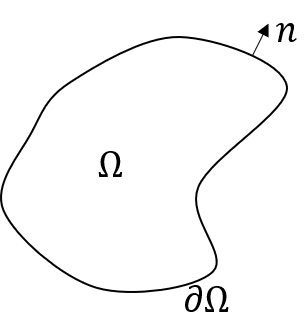
\includegraphics[scale=0.5]{./images/image1.png}
    \caption[区域符号示例]{区域符号示例}
    \label{fig:domain}
\end{figure}

现在考虑一个闭区域$\Omega$,$\Omega$的边界记为$\partial \Omega$,边界上的外法向记为
$n$,同时假定$\rho$ 和 $v$在 $\Omega$的一个开邻域内足够光滑。根据质量守恒,容易得到$\Omega$上质量的
变化率为$\partial \Omega$上质量的流出率和流入率之和。即
\begin{equation}
    \begin{split}
        \frac{d}{dt}\int_{\Omega} \rho(x,t)dx &= -\int_{\partial \Omega} \rho v \cdot n ds \\
        \int_{\Omega} \frac{\partial}{\partial t} \rho (x,t)dx &= -\int_{\Omega} div(\rho v)dx\nonumber\\
    \end{split}
\end{equation}
如果$\rho$在$\mathbb{R}^3$上都能达到足够光滑,那么由$\Omega$的任意性,可知
\begin{equation}
    \frac{\partial}{\partial t}\rho (x,t) + div(\rho v) = 0
\end{equation}

\subsection{欧拉视角下的动量守恒定律}
现在考虑闭区域$\Omega$上的动量变化。根据连续介质力学中的牛顿运动定律~\cite{gonzalez2008first},闭区域$\Omega$上的动量变化可以分为三部分,
第一部分为物质流入流出$\Omega$导致的动量变化,第二部分为作用在$\Omega$边界上的力导致的动量变化,第三部分为作用在$\Omega$内部物质上的力(一般为重力)产生的作用变化。
即
\begin{equation}
    \frac{d}{dt} \Big |_{t = t_0} \int_{\Omega} \rho v dx = -\int_{\partial \Omega} \rho v (v\cdot n) ds + \int_{\partial \Omega} \sigma \cdot n ds + \int_{\Omega} \rho g dx
\end{equation}
在(2.2)式中,$g$为重力加速度,$\sigma$为Cauthy应力~\cite{gonzalez2008first}。特别地,$\sigma$是一个三阶对称矩阵,其对称性来源于角动量守恒~\cite{marsden1994mathematical},我们将在2.4节中从另一个角度说明其对称性。

由于(2.2)式中$\Omega$选择的任意性,我们有
\begin{equation}
    \frac{\partial}{\partial t} \Big |_{t = t_0}(\rho v) = -div(\rho v^{T}v) + div(\sigma) + \rho g
\end{equation}

矩阵函数散度$div$定义如下:
\begin{equation}
    \begin{split}
        div &: C^1(\mathbb{R}^3;\mathbb{R}^{3\times 3}) \rightarrow C^1(\mathbb{R}^3;\mathbb{R}^3)\\
        &div(A)_i := \sum_j \partial_j A_{ij}\nonumber\\
    \end{split}
\end{equation}

(2.2)式变形为
\begin{equation}
    \frac{\partial}{\partial t} \Big |_{t = t_0}(\rho v) + div(\rho v^{T}v) = div(\sigma) + \rho g
\end{equation}


\section{拉格朗日视角下的动力学}
在上一节中,本文根据质量守恒和动量守恒得到了两个方程(方程(2.1)与方程(2.4)),非常重要的一点是,上述方程并没有使用任何
有关自然状态--材料在不施加外力的静止状态--的信息。在之后的章节中,我们将假定,$t=0$是处于自然状态,并且只考虑$t \ge 0$ 的情况。

假定在自然状态下($t = 0$),材料占据的空间为$\Omega_0 \subset \mathbb{R}^3$,此时也称$\Omega_0$为参考构型。对于任意给定的$t\in (0,+\infty)$,
此时材料占据的空间为$\Omega_t \subset \mathbb{R}^3$,相对于参考构型$\Omega_0$,称$\Omega_t$为当前构型。

拉格朗日视角和欧拉视角的区别主要是函数的定义域。在上一节中,我们所有函数的定义域都在$\mathbb{R}^3$上,而本节我们将把视角限制在材料上,例如对于任意时刻$t$,
有$\Omega_t$上的实值函数,$f(\cdot,t) :\Omega_t \rightarrow \mathbb{R} $。

\subsection{形变映射,形变梯度,速度}
为了描述材料相对于参考构型发生的形变,我们引入形变映射 $$\phi:\Omega_0 \times [0,+\infty) \rightarrow \mathbb{R}^3$$
形变映射同时也给出了物体的运动轨迹。
为了方便,我们记$\phi_t (x) = \phi(x,t)$,实际上我们还假定$\{ \phi_t(x): t\in \mathbb{R}\}$构成了一个单参数变换群,并且关于$t$至少二阶光滑,关于$X$至少有连续的一阶导数。

有了形变映射,我们可以引入对局部形变的刻画,即形变梯度$F(X,t):=\frac{\partial \phi_t(X)}{\partial X}$。实际上,形变梯度$F(X,t)$还可以视为$X$处切空间的映射,即
$$F(X,t):T_X \Omega_0 \rightarrow T_x \Omega_t$$
对于任意的$\partial_X \in T_X \Omega_0$, $\partial_x = F(X,t)[\partial_X] \in \Omega_t$,
即形变梯度将$X$点的切向量$\partial_X$经过平移起始点,旋转方向,拉伸长度后得到$x$点的切向量$\partial_x$,如图2.2所示。
\begin{figure}[htbp]
    \centering
    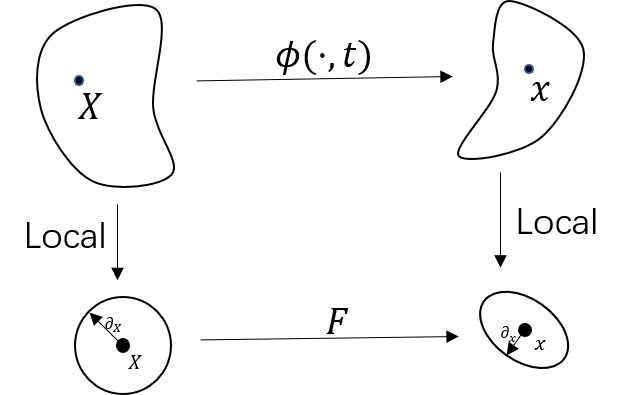
\includegraphics[scale=1.0]{./images/image2.png}
    \caption[形变与形变梯度]{形变与形变梯度}
    \label{fig:deformation gradient}
\end{figure}

同样的,形变映射作为单参数变换群,自然的导出速度的定义$V(X,t):= \frac{\partial \phi_t(X)}{\partial t}$。 值得注意的是,$V(X,t)$的定义域是在$\Omega_0$上,其值域
是一个起始点在$\Omega_t$上的一个三维列向量,其与欧拉视角下定义的速度关系为$V(X,t) = v(\phi_t(X),t)$,如果记$x = \phi_t(X)$,则$V(X,t) = v(x,t)$。

考察$F$关于时间的一阶导
\begin{equation}
    \begin{split}
        \frac{d}{dt}F(X,t) &= \frac{d}{dt}\frac{\partial}{\partial X}\phi_t\\
        &= \frac{\partial}{\partial X} \frac{d}{dt} \phi_t\\
        &= \frac{\partial}{\partial X} V(X,t)\\
        &= \frac{\partial v(\phi_t(X),t)}{\partial x}\frac{\partial \phi_t}{\partial X}\\
        &= \frac{\partial v(x,t)}{\partial x}\frac{\partial \phi_t}{\partial X}\\
        &= \nabla v \cdot F\nonumber
    \end{split}
\end{equation}
整理后我们得到$F$和$v$的关系
\begin{equation}
    \dot{F} = \nabla v \cdot F
\end{equation}


\subsection{拉格朗日视角下的质量守恒}
在引入了形变$\phi_t$之后,很自然的有$\hat{\Omega}_t = \{\phi_t(X):X\in \hat{\Omega}_0 \subset \Omega_0 \}$(简记为$\phi_t(\hat{\Omega}_0)$),且$\hat{\Omega}_t \subset \Omega_t$,
根据质量守恒,形变不会影响质量,即
$$\int_{\hat{\Omega}_0} \rho(x,0)dx = \int_{\hat{\Omega}_t} \rho(x,t)dx = \int_{\phi_t(\hat{\Omega}_0)} \rho(x,t)dx$$
如果我们将$\hat{\Omega}_t$的质量记为$M[\hat{\Omega}_t]$,则有$\frac{d}{dt}M[\hat{\Omega}_t] = 0$。而
\begin{equation}
    \begin{split}
        \frac{d}{dt} \int_{\phi_t(\hat{\Omega}_0)} \rho(x,t)dx &= \frac{d}{dt} \int_{\hat{\Omega}_0} \rho(\phi_t(X),t) det(F(X,t))dX\\
        &= \int_{\hat{\Omega}_0} \frac{d}{dt} [\rho(\phi_t(X),t) det(F(X,t))] dX \\
        &= 0\nonumber
    \end{split}
\end{equation}

记 $R(X,t):=\rho(\phi_t(X),t)$,$J(X,t):=det(F(X,t))$, 则根据$\hat{\Omega}_0$的任意性,有$\frac{d}{dt}[R(X,t)J(X,t)] = 0$,即
\begin{equation}
    R(X,t)J(X,t) = R(X,0)
\end{equation}
(2.6)式即为拉格朗日视角下的质量守恒方程。
\subsection{拉格朗日视角下的动量守恒}
在拉格朗日视角下,$\hat{\Omega}_{0}$的动量变化可以表示为作用在$\hat{\Omega}_{0}$边界上的力以及作用在$\hat{\Omega}_{0}$
内部的力之和。即
\begin{equation}
    \begin{split}
        \frac{d}{dt}\Big |_{t = t_0}\int_{\hat{\Omega}_0}R(X,0)V(x,t)dX = \int_{\partial \hat{\Omega}_{0}} P \cdot N dS + \int_{\hat{\Omega}_{0}} R(X,0) g dX
    \end{split}
\end{equation}
上式实际上对于任意的$\hat{\Omega}_0$成立,因此有以下
\begin{equation}
    R(X,0)\frac{\partial}{\partial t} V(X,t) = DIV(P) + Rg
\end{equation}
此处$DIV$是$\Omega_0$上的散度算子,为了与$\Omega_t$上进行区分记为大写。其中$P$是应力的另一种表述形式,称为First Piola–Kirchhoff应力~\cite{gonzalez2008first},其满足$\int_{\partial \hat{\Omega}_{0}} P \cdot N dS = \int_{\partial \hat{\Omega}_{t}} \sigma \cdot n ds$
我们将在下一节本构关系中更详细的给出$P$的计算方式以及与$\sigma$的关系。 

当然拉格朗日视角与欧拉视角下的动量守恒实际是等价的,我们接下来根据~\cite{gonzalez2008first}来说明其等价性,并且整理出一个更简洁的表达形式。
\begin{equation}
    \begin{split}
        \frac{d}{dt}\Big |_{t = t_0}\int_{\hat{\Omega}_0}R(X,0)V(x,t)dX &= \frac{d}{dt}\Big |_{t = t_0} \int_{\hat{\Omega}_0}R(X,t)v(\phi_t(X),t)J(X,t)dX\\
        &=\int_{\hat{\Omega}_0} \frac{d}{dt}\Big |_{t = t_0} [\rho(\phi_t(X),t)v(\phi_t(X),t)J(X,t)]dX\\
        &=\int_{\hat{\Omega}_0} \frac{d}{dt}\Big |_{t = t_0} [\rho(\phi_t(X),t)v(\phi_t(X),t)J(X,t)]dX\\
        &=\int_{\hat{\Omega}_0} v(\phi_{t_0}(X),t_0)\frac{d}{dt}\Big |_{t = t_0}[\rho(\phi_t(X),t) J(X,t)] \\
        &+ \rho(\phi_{t_0}(X),{t_0})J(X,t_0)\frac{d}{dt}\Big |_{t = t_0} v(\phi_{t_0}(X),t_0) dX\nonumber\\
        &=\int_{\hat{\Omega}_0}v(\phi_{t_0}(X),t_0)\frac{d}{dt}\Big |_{t = t_0}R(X,0) \\
        &+ \rho(\phi_{t_0}(X),{t_0})J(X,t_0)\frac{d}{dt}\Big |_{t = t_0} v(\phi_{t}(X),t)dX\\
        &=\int_{\hat{\Omega}_0}\rho(\phi_{t_0}(X),{t_0})J(X,t_0)\frac{d}{dt}\Big |_{t = t_0} v(\phi_{t}(X),t)dX\\
        &=\int_{\hat{\Omega}_{t_0}}\rho(x,t_0)\frac{d}{dt}\Big |_{t = t_0} v(\phi_{t,t_0}(x),t)dx\nonumber
    \end{split}
\end{equation}
这里$\phi_{t,t_0} = \phi_t \cdot \phi_{t_0}^{-1}$,带入(2.7)中就有
\begin{equation}
    \begin{split}
        \int_{\hat{\Omega}_{t_0}}\rho(x,t_0)\frac{d}{dt}\Big |_{t = t_0} v(\phi_{t,t_0}(x),t)dx = \int_{\hat{\Omega}_{t_0}} div(\sigma) dx + \int_{\hat{\Omega}_{t_0}} \rho g dx\nonumber
    \end{split}
\end{equation}
这里由于$\hat{\Omega}_{t_0}$为$\Omega_t$内的任意闭区域,因此
$$\rho(x,t_0)\frac{d}{dt}\Big |_{t = t_0} v(\phi_{t,t_0}(x),t) = div(\sigma) + \rho g$$

其中$$\frac{d}{dt}\Big |_{t = t_0} v(\phi_{t,t_0}(x),t) = \frac{\partial}{\partial t}\Big |_{t = t_0}v(x,t) + \sum_i \frac{\partial \phi_{t,t_0}^i}{\partial t}  \cdot \frac{\partial}{\partial x_i}v(x,t_0) = \frac{\partial}{\partial t}\Big |_{t = t_0}v(x,t) + v^T\nabla v$$
这里$\phi_{t,t_0}^i$为$\phi_{t,t_0}$的第$i$个分量。
此处引入材料时间导数$\frac{D}{Dt}f := \frac{\partial}{\partial t} f + v\nabla f $,将其代入上式中整理得
\begin{equation}
    \begin{split}
        \rho \frac{Dv}{Dt} = div(\sigma) + \rho g
    \end{split}
\end{equation}
该方程实际与(2.4)式等价,由于其更简洁的表述形式,我们之后将称(2.9)式为欧拉视角下的动量守恒。
$$\frac{\partial}{\partial t}(\rho v) + div(\rho v^{T}v) = div(\sigma) + \rho g$$
可考察方程的左端项
\begin{align*}
    \frac{\partial}{\partial t}(\rho v) + div(\rho v^{T}v) & = \rho \frac{\partial}{\partial t} v + v \frac{\partial}{\partial t} \rho + \rho v^T\nabla v + v div(\rho v)                           \\
                                                           & = \rho (\frac{\partial}{\partial t} v + v^T\nabla v) + v(\frac{\partial}{\partial t} \rho + div(\rho v))     & \text{第二项为质量守恒} \\
                                                           & = \rho \frac{Dv}{Dt}
\end{align*}
带入即知,(2.4)式是(2.8)式的展开。

\section{本构关系}
在前两节中,我们在动量守恒方程中引入了应力项,其决定了速度如何随着时间变化。本节我们将通过形变来给出
应变张量,其中应变张量和形变的函数关系被称为本构关系。事实上,本构关系直接决定了我们模拟的物体会表现出何种特质。

流体被认为是一种不可压缩的物质,用数学的语言就是说其形变梯度$F$满足$det(F)\equiv 1$,然而在实践中,为了更好的配合物质点法的使用,
我们从要求$det(F)\equiv 1$转变为使用形变能量密度来惩罚形变对体积的影响,$W(F):= \frac{\lambda}{2} (det(F) - 1)^2$。可以发现,对任意的$F\in \mathbb{R}^{3\times 3}, U\in SO_3$,始终有$W(UF) = W(F)$,
该特性被称为旋转不变性,根据诺特定理~\cite{takhtadzhian2008quantum},如果能量密度是旋转不变的,那么所得到的系统是角动量守恒的。

在有了能量密度函数,我们推导能量密度变化量和形变梯度的变化量之间的关系
\begin{equation}
    \begin{split}
        \delta W(F)&= \frac{\lambda}{2}\delta (det(F) - 1)^2\\
        &= \lambda (det(F) - 1) \delta(det(F) - 1)\\
        &= \lambda (det(F) - 1) \delta(det(F)) \nonumber\\
    \end{split}
\end{equation}
为了计算$\delta det(F)$,首先考察$\frac{d}{dt}\Big |_{t = 0}det(F + tI)$,由矩阵的特征多项式得
$$det(F + \epsilon I) = \epsilon ^n + \epsilon ^{n-1}Tr(F) + ... + det(F)$$
则等式两边同时除$\epsilon^n$得
$$det(\frac{1}{\epsilon}F + I) = 1 + \frac{1}{\epsilon} * Tr(F) + ... + \frac{1}{\epsilon^n} det(F)$$
此时将$t\neq 0$代入有
$$det(tF + I) = 1 + t Tr(F) + ... + t^ndet(F)$$
同时验证$t=0$可知上式恒成立。
因此$\frac{d}{dt}\Big |_{t = 0}det(tF + I) = tr(F)$,
现在对于任意的$t_0$以及$\mathbb{R}^{3 \times 3}$中通过$A(t_0)$(假设$A(t_0)$可逆)的一条光滑路径$A(t)$,我们有对应的通过$I$的路径
$A(t_0)^{-1}A(t)$,其对应的切向量为$A(t_0)^{-1}\frac{d}{dt}\Big |_{t=t_0}A(t)$,则
\begin{equation}
    \begin{split}
        \frac{d}{dt}\Big |_{t = t_0} det(A(t)) &= \lim_{h \to 0} \frac{det(A(t_0 + h)) - det(A(t_0))}{h}\\
        &=det(A(t)) \lim_{h\to 0} \frac{det(A(t_0)^{-1}A(t_0 + h)) -1}{h}\\
        &= det(A(t))tr(A(t_0)^{-1}\frac{d}{dt}\Big |_{t=t_0}A(t))\\
        &= det(A(t))A(t_0)^{-T}:\frac{d}{dt}\Big |_{t=t_0}A(t)
    \end{split}
\end{equation}
这里$A:B:=\sum_{i,j}A_{ij}B_{ij}$。

故$\delta det(F) = det(F) F^{-T}:\delta F$,代入$\delta W(F)$之中即有$$\delta W(F) = \lambda (det(F) - 1)det(F) F^{-T}:\delta F$$
其中$P = \lambda (det(F) - 1)det(F)F^{-T}$被称为First Piola–Kirchhoff应力,其与Cauthy应力$\sigma$的关系~\cite{marsden1994mathematical}为
$$J\sigma = PF^{T}$$
我们将在本小节最后给出该关系式的证明,代入可知柯西应力$\sigma = \lambda (det(F) - 1)I$。

这里的$W(F)$实际上只给出了物体的抗压缩性的性质,我们还需要给出表面张力的能量密度函数。根据~\cite{popinet2018numerical},表面能实际和物体表面积成正比,表面张力为表面能的梯度。那么我们首先可以得出
形变和表面能量的关系
\begin{equation}
    S(\phi_t) = k\int_{\phi_t (\partial \Omega_0)} ds
\end{equation}
为了更好的计算其梯度,我们对(2.11)式做一些处理。此处引入一些微分流形的记号~\cite{lee2013smooth},记$f^*$为$f$导出的拉回映射,$f_*$为推前映射,$ds,d\tilde{s}$分别为曲面$\partial \Omega_{t_0}, \partial \Omega_{t}$上的面积二形式,其为空间体积形式$dv$内乘法向的结果,
即$ds(X,Y) = dv(n,X,Y)$,我们记$ds = dv\odot n$,$ \tilde{p} = \phi_{t_0,t}(p)$,则对任意的$t \in[0, t_0),\tilde{X},\tilde{Y}\in T_{\tilde{p}}\Omega_t$有如下
\begin{equation}
    \begin{split}
        (\phi_{t_0,t}^*ds) (\tilde{X},\tilde{Y})& = (\phi_{t_0,t}^* (dv \odot n))(\tilde{X},\tilde{Y})\\
        &= ((\phi_{t_0,t}^* dv)\odot(\phi_{t_0,t}^* n))(\tilde{X},\tilde{Y})\\
        &= det(F(x;t_0,t))dv (<F^{-1}(x;t_0,t)n,\tilde{n}>\tilde{n} ,\tilde{X},\tilde{Y})\\
        &= det(F(x;t_0,t))<F^{-1}(x;t_0,t)n,\tilde{n}> dv(\tilde{n} ,\tilde{X},\tilde{Y})\\
        &= det(F(x;t_0,t))<n,F^{-T}(x;t_0,t)\tilde{n}>dv(\tilde{n} ,\tilde{X},\tilde{Y})
    \end{split}
\end{equation}
上式中$F(x;t_0,t) = \frac{\partial \phi_{t_0,t}(x)}{\partial x}$,$\tilde{n}$为$T_{\tilde{p}}\Omega_t$单位法向,$<\cdot,\cdot>$为空间内积,容易验证$F^{-T}(x;t_0,t)\tilde{n}$与$T_p\Omega_0$垂直,
故$<n,F^{-T}(x;t_0,t)\tilde{n}> = \Vert F^{-T}(x;t_0,t)\tilde{n}\Vert$, 即$\Vert F^{-T}(x;t_0,t)\tilde{n}\Vert n = F^{-T}(x;t_0,t)\tilde{n}$,那么有
$$(\phi_{t_0,t}^*ds) = det(F(x;t_0,t)) \Vert F^{-T}(x;t_0,t)\tilde{n}\Vert d\tilde{s}$$
则代入表面能表达式有
\begin{equation}
    \begin{split}
        S(\phi_{t_0}) &= k  \int_{\partial\Omega_{t_0}}ds\\
        &= k \int_{\phi_{t_0,t}(\partial\Omega_{t})} ds\\
        &= k \int_{\partial \Omega_t}  \phi_{t_0,t}^* ds\\
        &= k \int_{\partial \Omega_t} det(F(x;t_0,t)) \Vert F^{-T}(x;t_0,t)\tilde{n}\Vert d\tilde{s}\nonumber\\
    \end{split}
\end{equation}

至此,我们得到表面能的另一个表达形式
\begin{equation}
    \begin{split}
        S(\phi_{t_0}) = k \int_{\partial \Omega_t} det(F(x;t_0,t)) \Vert F^{-T}(x;t_0,t)\tilde{n}\Vert d\tilde{s}
    \end{split}
\end{equation}
(2.13)式将是表面张力离散化的基础。

最后,我们给出$J\sigma = PF^{T}$的证明,
\begin{align*}
    \int_{\partial \hat{\Omega}_{t}} \sigma \cdot n ds &= \int_{\phi_t (\partial \hat{\Omega}_{0})} \sigma\cdot n ds\\
    &= \int_{\partial \hat{\Omega}_0} \phi_t^*(\sigma\cdot n) (\phi_t^* ds)\\
    &= \int_{\partial \hat{\Omega}_0} \sigma\cdot n J \Vert F^{-T} N\Vert dS\\
    &= \int_{\partial \hat{\Omega}_0} \sigma F^{-T} \cdot F^{T}n J \Vert F^{-T} N\Vert dS\\
    &= \int_{\partial \hat{\Omega}_0} J\Vert F^{-T} N\Vert\sigma F^{-T} \cdot \frac{1}{\Vert F^{-T}N \Vert} N dS\\
    &= \int_{\partial \hat{\Omega}_0} J\sigma F^{-T} \cdot N dS\\
\end{align*}
而$\int_{\partial \hat{\Omega}_{0}} P \cdot N dS = \int_{\partial \hat{\Omega}_{t}} \sigma \cdot n ds$,因此$\int_{\partial \hat{\Omega}_0} J\sigma F^{-T} \cdot N dS = \int_{\partial \hat{\Omega}_0} P \cdot N dS$,
由于上式对任意$\partial \hat{\Omega}_0$成立,则$J\sigma F^{-T}= P$得$J\sigma = PF^{T}$。


\section{本章小结}
本章基于连续介质力学得到了一系列的控制方程
\begin{align*}
    &\frac{\partial}{\partial t}\rho (x,t) + div(\rho v) = 0 & \text{欧拉视角下的质量守恒方程} \\
    &R(X,t)J(X,t) = R(X,0) & \text{拉格朗日视角下的质量守恒方程} \\
    &\rho \frac{Dv}{Dt} = div(\sigma) + \rho g & \text{欧拉视角下的动量守恒方程}\\
    &R(X,0)\frac{\partial}{\partial t} V(X,t) = DIV(P) + Rg &\text{拉格朗日视角下的质量守恒方程}
\end{align*}

以上四个方程分别从两种视角分别等价的刻画了质量守恒和动量守恒,这两种视角也会在物质点法离散化的过程中体现出来。其次,通过整理得到
形变梯度更新方程~\cite{jiang2016material}
\begin{align*}
    \dot{F} = \nabla v \cdot F
\end{align*}
该方程将会在物质点法如何获得下一时刻的形变梯度中起到关键作用。最后,
我们给出了弱可压缩能量$W(F)=\lambda (J-1)^2$来刻画流体的特性,该能量也给出了First Piola–Kirchhoff应力和Cauthy应力的计算方式。
其次根据~\cite{popinet2018numerical}\cite{hyde2020implicit}得到表面能的另一个等价表达形式
$$S(\phi_{t_0}) = k \int_{\partial \Omega_{t_1}} det(F(x;t_0,t_1)) \Vert F^{-T}(x;t_0,t_1)\tilde{n}\Vert d\tilde{s}$$
该计算形式下,积分域不随着$\phi_{t_0}$变化而变化,为我们离散计算以及变分都带来了便利,而表面张力将由表面能变分获得,这一步我们将在离散化的过程(章节\ref{chap4})中来计算。







%literature
  \chapter{表面重建} \label{chap3}
\section{引言}
为了计算表面张力,我们需要一种能够从点云中获取表面和表面法向的方法。本文使用的方法是
使用粒子水平集方法[**]获得一个粗糙的一阶连续隐式曲面,并使用MarchingCube[**]算法重构表面网格。然而该网格
的质量只能做到一阶连续,计算得到的法向在面片之间并不连续,难以应用在表面张力所需的法向计算。本文在该网格
上进行泊松圆盘采样,然后结合已经存在的IPIA算法,提出一种新的快速重建算法以此获得一个二阶光滑
的隐式曲面,然后基于该隐式曲面来计算表面点云的法向。
\section{粒子水平集方法}
记$\mathcal{V}$为点云集合,$v\in \mathcal{V}$为粒子,记$d(x,v)\in \mathbb{R}$为空间上$x$的点到粒子$v$的距离,
则$\mathcal{S}(v) = \{x\in \mathbb{R}^3: d(x,v) = r\}$为半径为$r$,圆心在$v$的球,如图\ref{fig:particle levelset}左所示,蓝色圆圈为二位情况的$\mathcal{S}(v)$。
\begin{figure}[htbp]
    \centering
    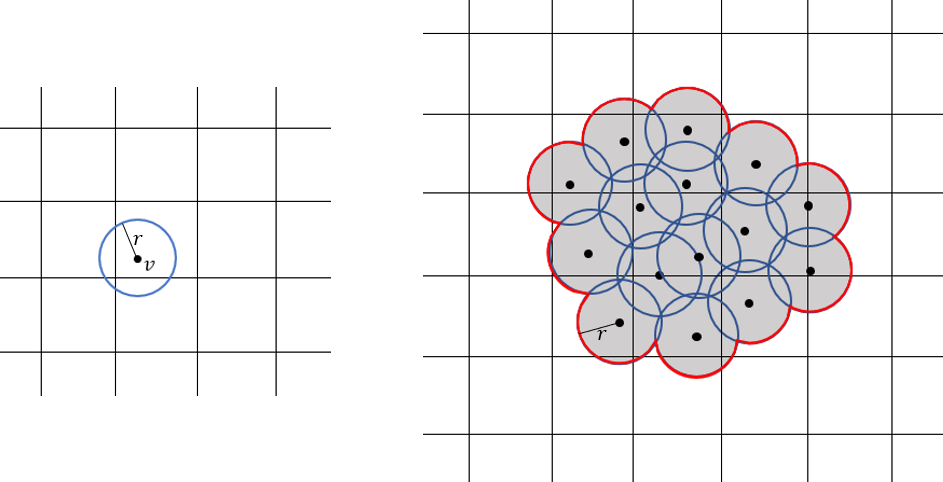
\includegraphics[scale=1.0]{./images/image3.png}
    \caption{二维情况$\mathcal{S}(v)$(左)与$\mathcal{S}(\mathcal{V})$(右)}
    \label{fig:particle levelset}
\end{figure}

记$d(x,\mathcal{V}):= \min \{ d(x,v): v\in \mathcal{V}\}$,则$\mathcal{S}(\mathcal{V}) = \{x\in \mathbb{R}^3: d(x,\mathcal{V}) = r\}$为点云的球外延边界。

如图\ref{fig:particle levelset}右所示,红色的外延边界为所求$\mathcal{S}(\mathcal{V})$。该红色边界初步确定了该点云的边界,灰色部分界定了物体内部。下一步我们将从利用红色边界和背景网格提取出
一个粗糙的网格。

\section{水平集网格提取}
Marching cube通常用于三维标量场的水平集的可视化,本文使用Marching cube算法来获取水平集的三角网格,在本文中我们的水平集为
$\mathcal{S}(\mathcal{V}) = \{x\in \mathbb{R}^3: d(x,\mathcal{V}) = r\}$。


\begin{figure}[htbp]
    \centering
    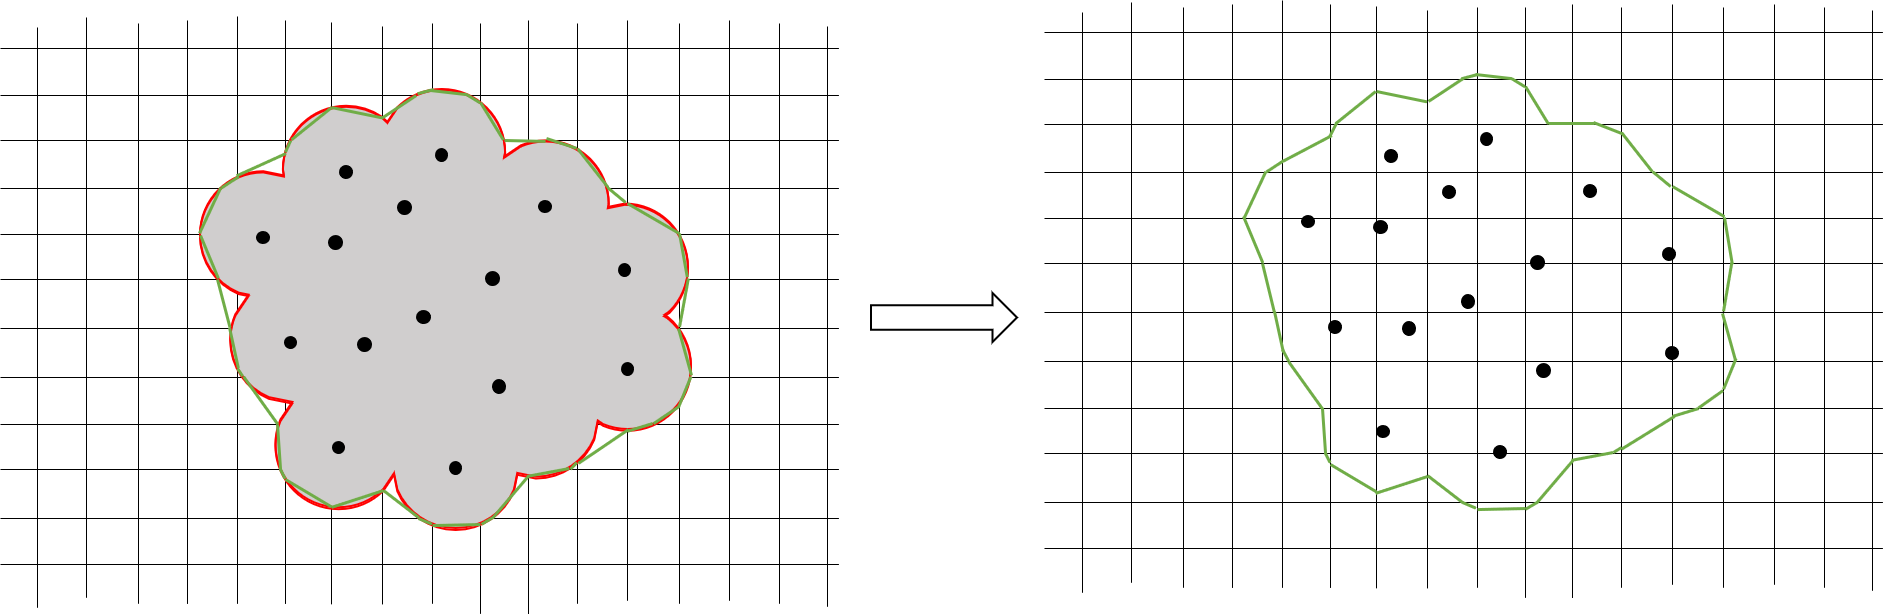
\includegraphics[scale=0.3]{./images/image7.png}
    \caption{二维点云轮廓提取图示}
    \label{fig:2D marching cube}
\end{figure}
\begin{figure}[htbp]
    \centering
    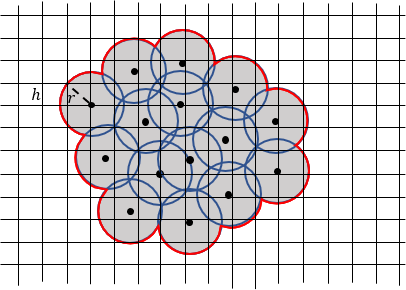
\includegraphics[scale=1.0]{./images/image5.png}
    \caption{二维情况的$r$与$h$的关系}
    \label{fig:grid and sphere}
\end{figure}

本小节我们的目标只是提取出一个大致的点云的表面轮廓,如图\ref{fig:2D marching cube}所示。我们首先将空间离散化成一个个均匀的立方体,我们称之为背景网格,并对每一个正方体格点放置一个标志符,默认为0,此处记立方体宽度为$h$,为了保证球能够覆盖到一个足够大的
面积,此处我们选择$r = \sqrt{3}h$,二维情况为$r = \sqrt{2}h$,具体如图\ref{fig:grid and sphere}所示。本文为了节省内存,
具体实现使用了八叉树数据结构。之后对每一个粒子操作,将粒子周围的格点做标记,如果格点距离该粒子半径不超过
$r$,则将格点标记为1,如此下来,所有的正方体格点都被标记为两种状态。之后我们对正方体按格点状态进行分类,由于每个格点有
两种状态,每个正方体有8个格点,如此一来便有$2^8 = 256$种状态,在合并旋转和对称的情况后,可以简化成15种,可以分类成如图\ref{fig:marching cube table}所示。
\begin{figure}[htbp]
    \centering
    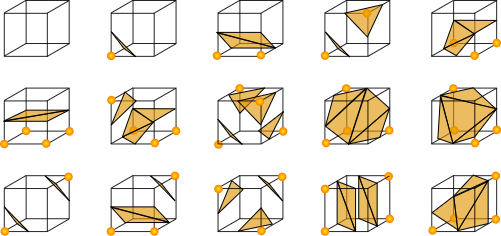
\includegraphics[scale=0.6]{./images/image6.png}
    \caption{Marching cube列表}
    \label{fig:marching cube table}
\end{figure}
之后我们再将网格顶点位置调整到合适的位置,并建立三角网格数据结构。具体的算法描述见\textbf{Algorithm \ref{alg:marching cube}}。
\begin{algorithm}
    \caption{Marching cube}
    \label{alg:marching cube}
    \begin{algorithmic}[1]
    \Require 点云集合$\mathcal{V}$,立方体宽度$h$
    \Ensure 三角网格位置集合$V$,面片集合$F$
    \State 准备空间网格数据结构(八叉树),并记$\mathcal{G}$为格点集合,$\mathcal{E}$为立方体的边集合,$\mathcal{C}$为立方体集合
    \State $state(g)\in \{0,1\}$为格点$g\in \mathcal{G}$的状态,初始化为0
    \State $P(e)\in \mathbb{R}^3$为边$e\in \mathcal{E}$上的一个顶点
    \State $r = \sqrt{3}h$
    \For{$v\in \mathcal{V}$}
        \For{$g \in \{g\in \mathcal{G}: \Vert g - v\Vert < r\}$}
            \State $state(g)$标记为1    
        \EndFor
    \EndFor    
    \For{$e \in \{e\in \mathcal{E}: e\text{两端格点状态相异}\}$}
      \State  取$e$状态为$1$的顶点记为$g_1$,状态为$0$的记为$g_0$
      \State 申请栈空间$p_{stack}$
      \For{$v \in \{v\in \mathcal{V}: \Vert g_1 - v\Vert < r\}$}
        \State 计算$\mathcal{S}(v)$与$e$的交点并压入$p_{stack}$中
      \EndFor
      \State 在$p_{stack}$中选取离$g_0$最近的点,并赋值给$P(e)$,同时将$P(e)$压入$V$中
    \EndFor
    \For{$c \in \mathcal{C}$}
        \State 匹配$c$所对应的Marching cube 列表中的状态
        \State 构造相应的三角面表$f_s$,顶点选为对应$P(e)$在$V$中得索引
        \State 将$f_s$其压入$F$中
    \EndFor
    \end{algorithmic}
\end{algorithm}


\textsf{在这里补点三维图,说明网格质量不行,只能一阶连续,法向不连续}


从实验结果的图中可以发现,Marching cube算法确实提取出了一个点云的边界轮廓,但是轮廓只能做到一阶连续,法向明显不连续,同时其三角网格质量无法
无法保证,甚至可以明显看出在一些尖锐地方,网格质量极差,上述的问题给我们计算表面张力带来了很大的阻碍。

\section{LSIPIA}
为了解决法向不连续的问题以及网格质量差的问题,我们使用二阶连续的隐式曲面来逼近三角网格,因此隐式曲面的法向一阶连续。

\subsection{隐式曲面的渐进迭代逼近}
我们首先给出隐式曲面重建问题,给定一个无序点集$\mathcal{V} = \{v_i = (v_i^1,v_i^2,v_i^3)\}_{i = 1}^n$以及点
上的单位法向量$\mathcal{N} = \{n_i = (n_i^1, n_i^2, n_i^3)\}_{i = 1}^n$,寻找一个函数$f(x^1,x^2,x^3)$使得
$f(x^1,x^2,x^3)$的$0$水平集拟合该组无序点集$\mathcal{V}$。以数学的表达形式即为
\begin{equation}
    \begin{split}
        \min_f\sum_{i = 1}^{n} f(v_i^1,v_i^2,v_i^3)^2       
    \end{split}
\end{equation}
为了让问题可解,我们选择$f$为有限个张量积B-样条基函数的线性组合,即$$f(x^1,x^2,x^3) = \sum_{i = 1}^{N_x}\sum_{j = 1}^{N_y}\sum_{k = 1}^{N_z} C_{ijk}B_i(x^1)B_j(x^2)B_k(x^3)$$
这里我们选择二阶B-样条基函数,其中二阶标准B-样条函数
$$B(x) = \begin{cases}
    \frac{3}{4} - \left | x \right | ^2  & 0 \leq \left | x \right | < \frac{1}{2}\\
    \frac{1}{2}(\frac{3}{2} - \left | x \right |)^2 & \frac{1}{2}\leq \left | x \right | <\frac{3}{2}\\
    0 & \frac{3}{2} \leq \left | x \right |
   \end{cases}$$
如图\ref{fig: standard B-spline basis}所示,这里$B_i(x) := B(\frac{1}{h}(x - x_i))$,这里的$x_i$本文选取为空间立方体网格格点坐标的一个分量,$h$为立方体宽度。
\begin{figure}[htbp]
    \centering
    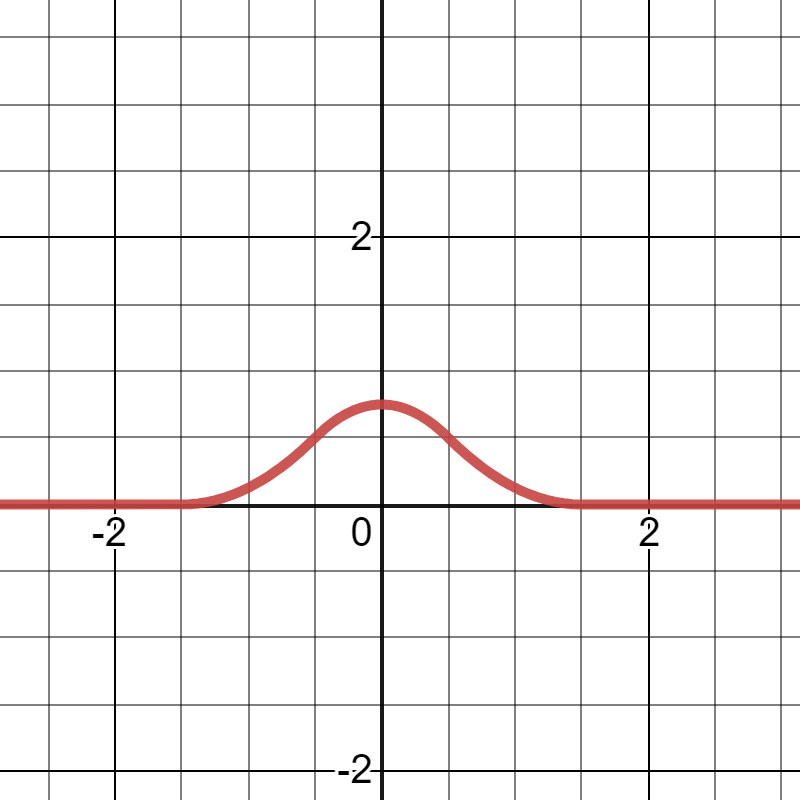
\includegraphics[scale=0.2]{./images/image8.png}
    \caption{二次标准B-样条基函数}
    \label{fig: standard B-spline basis}
\end{figure}
则最小化问题(3.2)转化成
\begin{equation}
    \begin{split}
        \min_{C_{ijk}}E(C_{111},C_{112},...,C_{N_xN_yN_z}):=\frac{1}{2}\sum_{i = 1}^{n} f(v_i^1,v_i^2,v_i^3)^2 
    \end{split}
\end{equation}
这里$C_{ijk}$张量积B-样条系数。

我们记三变量B-样条基函数为$B_{ijk}(x^1,x^2,x^3) = B_i(x^1)B_j(x^2)B_k(x^3)$,则上述问题变为
\begin{equation}
    \begin{split}
        &\min_{C_{ijk}}E(C_{111},C_{112},...,C_{N_xN_yN_z}):= \frac{1}{2}\sum_{r = 1}^{n} (\sum_{ijk}C_{ijk}B_{ijk}(v_r^1,v_r^2,v_r^3))^2 \\
        &\Leftrightarrow \delta E(\{C_{ijk}\}) = 0\\
        &\Leftrightarrow \delta (\frac{1}{2}\sum_{r = 1}^{n} (\sum_{ijk}C_{ijk}B_{ijk}(v_r^1,v_r^2,v_r^3))^2) = 0\\
        &\Leftrightarrow \sum_{r = 1}^{n} \sum_{ijk} \sum_{uvw}C_{ijk}B_{ijk}(v_r^1,v_r^2,v_r^3)B_{uvw}(v_r^1,v_r^2,v_r^3)\delta C_{uvw} = 0\\
        &\Leftrightarrow \sum_{r = 1}^n \sum_{ijk} C_{ijk} B_{ijk}(v_r^1,v_r^2,v_r^3)B_{uvw}(v_r^1,v_r^2,v_r^3) = 0
    \end{split}
\end{equation}
我们将$\{B_{111},B_{112},...,B_{11N_z},...,B_{1Ny1},...B_{N_xN_yN_z}\}$以字典序排列,这样我们可配置如下矩阵
\begin{align*}
    \mathbf{B} = \begin{bmatrix}
        B_{111}(v_1^1,v_1^2,v_1^3) & B_{112}(v_1^1,v_1^2,v_1^3) &...& B_{N_xN_yN_z}(v_1^1,v_1^2,v_1^3)\\
        B_{111}(v_2^1,v_2^2,v_2^3) & B_{112}(v_2^1,v_2^2,v_2^3) &...& B_{N_xN_yN_z}(v_2^1,v_2^2,v_2^3)\\
         \vdots & \vdots & & \vdots\\
        B_{111}(v_r^1,v_r^2,v_r^3) & B_{112}(v_r^1,v_r^2,v_r^3) &...& B_{N_xN_yN_z}(v_r^1,v_r^2,v_r^3)\\
    \end{bmatrix}
\end{align*}
同样对于$\{C_{111},...,C_{N_xN_yN_z}\}$我们有
\begin{align*}
    \mathbf{C} = \begin{bmatrix}
        C_{111} \\
        \vdots \\
        C_{N_xN_yN_z}\\
    \end{bmatrix}
\end{align*}
代入(3.3)最后一个式子中,我们可以得到一个紧凑的形式
$$\mathbf{B}^T \mathbf{B} \mathbf{C} = 0$$
然而,在实践中以上线性系统并非有唯一解,并且有平凡解($\mathbf{C} = 0$)。为了避免陷入平凡解,我们添加法向扰动。
我们利用本小节开头提到的每一点上的法向信息$\mathcal{N}$,我们利用法向取一些偏移点$\mathcal{Q} = \{q_i = v_i + \epsilon n_i: v_i \in \mathcal{V}, n_i \in \mathcal{N}\}$。
然后尽可能要求$f(q_i) = \epsilon, i = 1,2,3,...n$。据此我们修改(3.3)中的优化问题,
\begin{equation}
    \begin{split}
        &\min_{C_{ijk}}E(C_{111},C_{112},...,C_{N_xN_yN_z}):= \frac{1}{2}\sum_{r = 1}^{n} [ (\sum_{ijk}C_{ijk}B_{ijk}(v_r^1,v_r^2,v_r^3))^2 + (\epsilon - \sum_{ijk}C_{ijk}B_{ijk}(q_r^1,q_r^2,q_r^3))^2]\\
        &\Leftrightarrow \sum_{r = 1}^n (\sum_{ijk}C_{ijk} B_{ijk}(v_r^1,v_r^2,v_r^3)B_{uvw}(v_r^1,v_r^2,v_r^3) - ( \epsilon - \sum_{ijk} C_{ijk}B_{ijk}(q_r^1,q_r^2,q_r^3) )B_{uvw}(q_r^1,q_r^2,q_r^3))\\
    \end{split}
\end{equation}

\begin{align*}
    \mathbf{B} = \begin{bmatrix}
        B_{111}(v_1^1,v_1^2,v_1^3) & B_{112}(v_1^1,v_1^2,v_1^3) &...& B_{N_xN_yN_z}(v_1^1,v_1^2,v_1^3)\\
        B_{111}(v_2^1,v_2^2,v_2^3) & B_{112}(v_2^1,v_2^2,v_2^3) &...& B_{N_xN_yN_z}(v_2^1,v_2^2,v_2^3)\\
         \vdots & \vdots & & \vdots\\
        B_{111}(v_r^1,v_r^2,v_r^3) & B_{112}(v_r^1,v_r^2,v_r^3) &...& B_{N_xN_yN_z}(v_r^1,v_r^2,v_r^3)\\
        B_{111}(q_1^1,q_1^2,q_1^3) & B_{112}(q_1^1,q_1^2,q_1^3) &...& B_{N_xN_yN_z}(q_1^1,q_1^2,q_1^3)\\
        B_{111}(q_2^1,q_2^2,q_2^3) & B_{112}(q_2^1,q_2^2,q_2^3) &...& B_{N_xN_yN_z}(q_2^1,q_2^2,q_2^3)\\
        \vdots & \vdots & & \vdots\\
        B_{111}(q_r^1,q_r^2,q_r^3) & B_{112}(q_r^1,q_r^2,q_r^3) &...& B_{N_xN_yN_z}(q_r^1,q_r^2,q_r^3)\\
    \end{bmatrix}
\end{align*}
如果再记
\begin{align*}
    \mathbf{b} = \begin{bmatrix}
        0\\
        \vdots\\
        0\\
        \epsilon \\
        \vdots \\
        \epsilon
    \end{bmatrix}
\end{align*}
其中$\mathbf{b}$的前$n$项为$0$,后$n$项为$\epsilon$。则(3.4)式可以写成紧凑的形式
\begin{equation}
    \mathbf{B}^T ( \mathbf{b} - \mathbf{B} \mathbf{C}) = 0    
\end{equation}
求解该线性系统,我们使用迭代法求解,与IPIA[**]不同,我们的迭代格式为
\begin{equation}
\mathbf{C}^{\alpha + 1} = \mathbf{C}^{\alpha} + \Lambda \mathbf{B}^T(\mathbf{b} - \mathbf{B}\mathbf{C}^{\alpha}) , \alpha = 0,1,2...
\end{equation}
这里$\Lambda$为
\begin{equation}
    \begin{split}
        \begin{bmatrix}
            \frac{1}{\sum_{r = 1}^n B_{111}(v_r) +B_{111}(q_r)} & 0 & ... & 0\\
            0 & \frac{1}{\sum_{r = 1}^n B_{112}(v_r) +B_{112}(q_r)} & ... & 0\\
            \vdots & \vdots & ... & \vdots \\
            0 & 0 & ... & \frac{1}{\sum_{r = 1}^n B_{N_xN_yN_z}(v_r) +B_{N_xN_yN_z}(q_r)} \\
        \end{bmatrix}
    \end{split}
\end{equation}
这里$B_{ijk}(x) = B_{ijk}(x^1,x^2,x^3)$,并假设$\Lambda$可逆(即$\forall ijk ,\sum_{r = 1}^n B_{ijk}(v_r) +B_{ijk}(q_r) \neq 0$),否则认为有某个节点$ijk$满足$\sum_{r = 1}^n B_{ijk}(v_r) +B_{ijk}(q_r) = 0$,由于B-样条基函数非负,则$B_{ijk}(v_r) = B_{ijk}(q_r) = 0$,我们可以去掉该节点,同时去掉对应的$\mathbf{B}$和$\mathbf{C}$对应的行,其并不影响点云附近的隐式曲面构建。
所以我们不妨假定$\Lambda$可逆。有关收敛性的证明,详见[**]。本迭代格式相较于IPIA格式最大的优势就是内存占用少,可高度并行,我们从\textbf{Algorithm \ref{alg:LSIPIA}}来分析这一点。
我们可以发现\textbf{Algorithm \ref{alg:LSIPIA}}在第4行,第15行,第22行对应的循环可高度并行。同时需要的额外内存为储存在每个格点$\mathcal{G}$上的$C_{ijk}$,$\lambda_{ijk}$,$\Delta_{ijk}$。而这一点,我们将在下一节中
说明里所需的额外内存可以借用物质点法中的数据结构完成,也就是说LSIPIA的优势为可复用物质点法的数据结构,同时可以高度并行。

[***************************补充实验数据****************************]
\begin{algorithm}
    \caption{LSIPIA}
    \label{alg:LSIPIA}
    \begin{algorithmic}[1]
    \Require 点云位置$\mathcal{V}$,点云法向$\mathcal{N}$,背景网格格点集合$\mathcal{G}$,指定迭代次数$LoopTimes$
    \Ensure 隐式曲面$f(x) = \sum_{ijk} C_{ijk}B_{ijk}(x)$,即输出参数值$C_{ijk}$
    \State 初始化$\forall ijk,C_{ijk} = 0$
    \State 初始化$\forall ijk,\lambda_{ijk} = 0$
    \State 初始化偏移量$\epsilon$
    \For{$r \in \#\mathcal{V}$}
        \State 预计算下标为$I = \{ijk : v_r \in supp(B_{ijk})\}$的张量积B-样条函数,储存为$B_{ijk}(v_r)$
        \For{$ijk \in I$}
            \State $\lambda_{ijk} \leftarrow \lambda_{ijk} + B_{ijk}(v)$
        \EndFor
        \State $v_{\epsilon r} \leftarrow v_r + \epsilon n_r$
        \State 预计算下标为$I_{\epsilon} = \{ijk : v_{\epsilon r} \in supp(B_{ijk})\}$的张量积B-样条函数,储存为$B_{ijk}(v_{\epsilon r})$
        \For{$ijk \in I_{\epsilon}$}
            \State $\lambda_{ijk} \leftarrow \lambda_{ijk} + B_{ijk}(v_{\epsilon r})$
        \EndFor
    \EndFor
    
    \For{$ijk \in \mathcal{G}$}
        \If {$\lambda_{ijk}\neq 0$} 
            \State $\lambda_{ijk}\leftarrow \frac{1}{\lambda_{ijk}}$
        \EndIf
    \EndFor

    \State 初始化$\forall ijk,\Delta_{ijk} = 0$
    \For{$i = 1,\dots,LoopTimes$}
        \For{$r \in \#\mathcal{V}$}
            \State 预计算下标为$I = \{ijk : v_r \in supp(B_{ijk})\}$的张量积B-样条函数,储存为$B_{ijk}(v_r)$
            \State $res = 0$
            \For{$ijk \in I$}
                \State $res \leftarrow res + B_{ijk}(v_r)$ 
            \EndFor
            \State $\delta_r = 0 - res$
            \For{$ijk \in I$}
                \State $\Delta_{ijk}\leftarrow \Delta_{ijk} + \delta_r \cdot B_{ijk}(v_r)$ 
                \State 重置$\Delta_{ijk}$为0
            \EndFor
        \EndFor
    \EndFor

    \end{algorithmic}
\end{algorithm}

\subsection{快速法向计算}
在完成\textbf{Algorithm \ref{alg:LSIPIA}}之后,我们获得了一个二阶连续的隐式曲面。即
\begin{equation}
    f(x) = \sum_{ijk} C_{ijk}B_{ijk}(x)
\end{equation}
获取法向我们可以直接计算其梯度$\nabla f$,我们首先分析计算一个点上的梯度所需要的代价。
首先根据张量积B-样条函数的定义$B_{ijk}(x) = B_i(x^1) * B_j(x^2) * B_k(x^3)$,如果选取的为二次样条,则在二维情况下
其能够覆盖到点$x$的基函数如图\ref{fig:2D basis},所以能够覆盖到点$x$的坐标个点为$I = \{ij: i = i_0 + k, j = i_0 + l, \text{其中}k, l \in \{0,1,2\}\}$。
\begin{figure}[htbp]
    \centering
    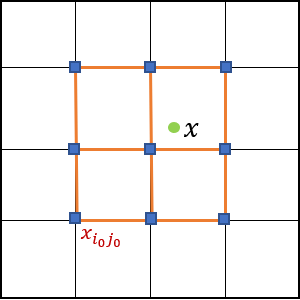
\includegraphics[scale=1.0]{./images/image9.png}
    \caption{蓝色正方形为其紧支集能够覆盖$x$的自由度,$x_{i_0j_0}$为左下角格点坐标}
    \label{fig:2D basis}
\end{figure}

而
\begin{equation}
    \begin{split}
        \nabla f &= \sum_{ijk} C_{ijk} \nabla B_{ijk}(x)\\
        &= \sum_{ijk} C_{ijk} \nabla (B_i(x^1)B_j(x^2)B_k(x^3))\\
        &= \sum_{ijk} C_{ijk} (\partial_1 B_i(x^1) \cdot B_j(x^2)B_k(x^3), B_i(x^1)\partial_2 B_j(x^2)\cdot B_k(x^3), B_i(x^1)B_j(x^2)\partial_3B_k(x^3))\\
    \end{split}
\end{equation}
可以发现要计算$x$点的梯度$\nabla f$, 我们需要计算的有$B_i(x^r),\partial_r B_i(x^r), i \in \{0,1,2\}, r \in \{1,2,3\}$,其中样条阶数越高,计算$\partial_r B_i(x^r)$代价越大,并且$\partial_r B_i(x^r)$为分段函数,故在不同的$r$之间不可能做到单指令多数据流并行,同样在拼装
$\nabla B_{ijk}(x)$时每一个维度需要单独的计算。基于这些缺点,我们提出另一个近似法向的计算方法。这里我们使用移动加权最小二乘来逼近格点系数,我们将会看到在
格点张量积B-样条基下,移动加权最小二乘将有惊人的简单形式。

我们寻求的近似目标函数为$f_y (x;c) = f(y) + c^T(x - y)$,能量函数设计如下
\begin{equation}
    \begin{split}
        E_y(c) = \frac{1}{2} \sum_{ijk} B_{ijk}(y)(f_y(x_{ijk};c) - C_{ijk})^2
    \end{split}
\end{equation}
对上式取极小我们得到
\begin{equation}
    \begin{split}
        0& = \frac{\partial}{\partial c} E_y(c)\\
        &= \frac{\partial}{\partial c} \frac{1}{2}\sum_{ijk} B_{ijk}(y)(f(y) + c^T (x_{ijk} - y) - C_{ijk})^2\\
        &= \sum_{ijk} B_{ijk}(y)(f(y) + c^T (x_{ijk} - y) - C_{ijk}) (x_{ijk} - y)^T\\
        &= \sum_{ijk} B_{ijk}(y)(f(y) - C_{ijk})(x_{ijk} - y)^T + c^T\sum_{ijk}B_{ijk}(y)(x_{ijk} - y)(x_{ijk} - y)^T\\ 
    \end{split}
\end{equation}
则 $$\sum_{ijk} B_{ijk}(y) (C_{ijk} - f(y)) (x_{ijk} - y) = [\sum_{ijk}B_{ijk}(y)(x_{ijk} - y)(x_{ijk} - y)^T]c $$
当然我们要计算$c$我们得到如下式子
\begin{equation}
    c = [\sum_{ijk}B_{ijk}(y)(x_{ijk} - y)(x_{ijk} - y)^T]^{-1} \cdot \sum_{ijk} B_{ijk}(y) (C_{ijk} - f(y)) (x_{ijk} - y)
\end{equation}
这里(3.12)式要成立的条件为$[\sum_{ijk}B_{ijk}(y)(x_{ijk} - y)(x_{ijk} - y)^T]$可逆,我们接下来证明该矩阵可逆。

此处我们记$A = \sum_{ijk}B_{ijk}(y)(x_{ijk} - y)(x_{ijk} - y)^T$。首先我们计算$A$的非对角项即$A_{uv}, u\neq v\text{其中} u,v \in \{1,2,3\}$,这里再记$w \in \{1,2,3\}\text{且} w \notin \{u,v\} $。
即
\begin{equation}
    \begin{split}
        A_{uv} &= \sum_{i_1 i_2 i_3} B_{i_1 i_2 i_3}(y) (x_{i_1 i_2 i_3}^u - y^u)(x_{i_1 i_2 i_3}^v - y^v)\\
        & = \sum_{i_u i_v i_w} B_{i_u}(y^u)B_{i_v}(y^v)B_{i_w}(y^w) (x_{i_u i_v i_w}^u - y^u)(x_{i_u i_v i_w}^v - y^v)\\
        & = \sum_{i_w}B_{i_w}(y^w)(\sum_{i_u}B_{i_u}(y^u)(x_{i_u i_v i_w}^u - y^u))(\sum_{i_v}B_{i_v}(y^v)(x_{i_u i_v i_w}^v - y^v))\\
        & =  \sum_{i_w}B_{i_w}(y^w)(\sum_{i_u}B_{i_u}(y^u)x_{i_u i_v i_w}^u - y^u\sum_{i_u}B_{i_u}(y^u))(\sum_{i_v}B_{i_v}(y^v)x_{i_u i_v i_w}^v - y^v\sum_{i_v}B_{i_v}(y^v))
    \end{split}
\end{equation}

这里我们注意到B-样条基函数的单位分解性$\sum_i B_i(x) = 1$以及线性还原性$\sum_i x_iB_i(x) = x$,带入到
(3.13)式中我们有
$$\sum_{i_w}B_{i_w}(y^w)(\sum_{i_u}B_{i_u}(y^u)x_{i_u i_v i_w}^u - y^u\sum_{i_u}B_{i_u}(y^u))(\sum_{i_v}B_{i_v}(y^v)x_{i_u i_v i_w}^v - y^v\sum_{i_v}B_{i_v}(y^v)) = 0$$
因此$u\neq v\text{时}A_{uv} = 0$,即$A$为对角阵。

接下来考察$u = v$时$A_{uv}$的值,而
\begin{equation}
    \begin{split}
        A_{uu} &= \sum_{i_1 i_2 i_3} B_{i_1 i_2 i_3}(y) (x_{i_1 i_2 i_3}^u - y^u)^2\\
            &= \sum_{i_u i_v i_w} B_{i_u}(y^u)B_{i_v}(y^v)B_{i_w}(y^w)(x_{i_1 i_2 i_3}^u - y^u)^2\\
            &= \sum_{i_u} B_{i_u}(y^u) (x_{i_1 i_2 i_3}^u - y^u)^2 \sum_{i_v}B_{i_v}(y^v)\sum_{i_v}B_{i_w}(y^w)\\
            &= \sum_{i_u} B_{i_u}(y^u) (x_{i_1 i_2 i_3}^u - y^u)^2\\ 
    \end{split}
\end{equation}
接下来我们仔细的计算$B_{i_u}(y^u)$,其中紧支集包含$y^u$的基函数如图\ref{fig:affected basis}所示。
\begin{figure}[htbp]
    \centering
    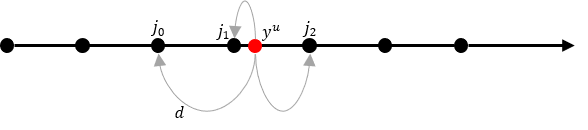
\includegraphics[scale=1.0]{./images/image10.png}
    \caption{$B_{j_0}(y^u), B_{j_1}(y^u), B_{j_2}(y^u)$为紧支集覆盖$y^u$的基函数,最左端为$j_0$,与$y^u$距离为$d$}
    \label{fig:affected basis}
\end{figure}



%literature
  \chapter{数值方法} \label{chap4}
\section{引言}
在前文给出连续的控制方程,以及表面重建方法后,本章将离散化连续控制方程,以及针对
流体表面张力给出一个物质的离散化方式,同时给出一个计算流水线将表面重建方法整合到物质点法中来完成我们的模拟。
\section{离散控制方程}
我们将使用伽辽金方法离散化控制方程,首先我们先将第一章中的动量强形式方程转换成弱形式,然后根据弱形式选取基函数以及
对应的离散方法用于数值计算。此处我们回顾动量守恒方程的欧拉形式和拉格朗日形式,
\begin{align*}    
    &\rho \frac{Dv}{Dt} = div(\sigma) + \rho g & \text{欧拉视角}\\
    &R(X,0)\frac{\partial}{\partial t} V(X,t) = DIV(P) + Rg &\text{拉格朗日视角}
\end{align*}
其中$v(x,t) = V(X,t), x = \phi(X,t)$。如果我们从拉格朗日视角来观察方程的左侧(时间变化项),从欧拉视角来观察方程的右侧(空间变化项),
那么我们有如下混合欧拉拉格朗日形式的方程
\begin{align*}
    &R(X,0)\frac{\partial}{\partial t} V(X,t) = div(\sigma) + \rho g & \text{混合欧拉拉格朗日视角}\\ 
\end{align*}
\subsection{时间离散化}
在混合欧拉拉格朗日视角中,左端项为$R(X,0)\frac{\partial}{\partial t}V(X,t)$,相对于欧拉视角下$\rho \frac{Dv}{Dt}$中的材料时间导数
$\frac{D}{Dt} = \frac{\partial}{\partial t} + v\cdot \nabla$,显然有更容易的离散方式,这也是时间变化项选择拉格朗日描述的原因。
此处我们使用有限差分来离散速度有关时间的变化。
\begin{align*}
    \frac{\partial}{\partial t} V(X,t) \approx \frac{V(X,t^{n+1}) - V(X,t^n)}{\Delta t}
\end{align*}

同样的,在拉格朗日视角下的离散化可以转换为欧拉视角下的离散化,这里记$x^{n} := \phi_{t^n}(X)$, $\hat{x}^{n+1} := \phi_{t^{n+1},t^n}(x^n)$,同时
$v^n(x^n) := v(x^n,t^n), \hat{v}^{n+1}(x^n) := v(\phi_{t^{n+1},t^n}(x^n))$,因此以上差分格式可以写成
\begin{align*}
    \frac{\partial}{\partial t} V(X,t) \approx \frac{\hat{v}^{n+1}(x^n) - v^n(x^n)}{\Delta t}
\end{align*}
值得注意的是,$\hat{v}^{n+1}(x^n)$与$v^n(x^n)$都是在$\Omega^{t^n} = \phi_{t^n}(\Omega^0)$上定义的,因此该离散形式既可在欧拉视角下表示,同时也可以在
拉格朗日视角下表示。
\subsection{弱形式}
将左端形式带入欧拉视角中,我们有如下
\begin{align*}
    \rho(x^n,t^n)\frac{\hat{v}^{n+1}(x^n) - v^n(x^n)}{\Delta t} = div(\sigma) + \rho g
\end{align*}
为了将表面张力融入方程中,我们补充边界条件如下
\begin{align*}
    \rho(x^n,t^n)\frac{\hat{v}^{n+1}(x^n) - v^n(x^n)}{\Delta t} &= div(\sigma) + \rho g \\
    \sigma n &= t, x^n \in \partial \Omega^{t^n}\\
\end{align*}
上述方程以弱形式表示我们有,这里$w$选取为空间上具有紧支集的测试函数
\begin{align*}
    \int_{\Omega^{t^n}}\rho(x,t^n)\frac{\hat{v}^{n+1}(x) - v^n(x)}{\Delta t}\cdot wdx &= \int_{\Omega^{t^n}} div(\sigma)\cdot w dx + \int_{\Omega^{t^n}}\rho g\cdot w dx\\
    \sigma n &= t, x \in \partial \Omega^{t^n}\\   
\end{align*}
现在我们处理右端的散度项,由格林公式~\cite{evans1998partial}得
\begin{align*}
    \int_{\Omega^{t^n}} div(\sigma)\cdot w dx &= \int_{\partial \Omega^{t^n}}w\cdot (\sigma n) ds - \int_{\Omega^{t^n}} \sigma : \nabla w dx\\
        &= \int_{\partial \Omega^{t^n}}w\cdot t ds - \int_{\Omega^{t^n}} \sigma :\nabla w dx
\end{align*}
我们先计算$\int_{\partial \Omega^{t^n}}\sigma : \nabla w dx$部分。回顾流体弱可压缩模型获得的柯西应力$$\sigma = \lambda (det(F) - 1)I$$带入可得
$\int_{\partial \Omega^{t^n}} \lambda (det(F) - 1) I:\nabla w dx$。
将上式整合我们得到
\begin{align*}
    \int_{\Omega^{t^n}}\rho(x,t^n)\frac{\hat{v}^{n+1}(x) - v^n(x)}{\Delta t}\cdot wdx &= \int_{\partial \Omega^{t^n}} w\cdot t ds - \int_{\Omega^{t^n}} \sigma:\nabla w dx
\end{align*}
为了计算表面张力项,回顾我们在第一章得到的表面张力计算公式
$$S(\phi_{t}) = k \int_{\partial \Omega_{t^n}} det(F(x;t,t^{n})) \Vert F^{-T}(x;t,t^{n})\tilde{n}\Vert d\tilde{s}$$
我们对其变分将获得流体表面上的表面张力场。为了方便,我们先记$\tilde{F} = F(x;t,t^n)$,以及$\Psi(\tilde{F}) = det(\tilde{F})\Vert \tilde{F}^{-T}\tilde{n} \Vert$,则
\begin{align}
    \delta \Psi(\tilde{F}) &= \delta(det(\tilde{F})\Vert \tilde{F}^{-T}\tilde{n} \Vert) \nonumber\\
    &= \delta[det(\tilde{F})] \Vert \tilde{F}^{-T} \tilde{n} \Vert + det(\tilde{F})\delta \Vert \tilde{F}^{-T}\tilde{n} \Vert \nonumber\\
    &= det(\tilde{F})\tilde{F}^{-T}:\delta \tilde{F} \cdot \Vert \tilde{F}^{-T}\tilde{n}\Vert + det(\tilde{F})\delta \Vert \tilde{F}^{-T} \tilde{n} \Vert
\end{align}
这里第三行我们使用了第二章提到的行列式求导结果$\delta det(F) = det(F)F^{-T}:\delta F$,接下来我们处理上述等式的右端项
$\delta \Vert \tilde{F}^{-T}\tilde{n}\Vert$。这里注意到$\Vert V \Vert^2 = V^TV$,因此我们有$2\Vert V\Vert \delta \Vert V \Vert = 2V^T\delta V$。
同时$A^{-1}A = I$,从这里我们由$\delta A^{-1} A + A^{-1}\delta A = 0$,整理得到$\delta (A^{-1}) = - A^{-1}\delta A A^{-1}$。那么我们由
\begin{align*}
    \delta \Vert \tilde{F}^{-T}\tilde{n}\Vert &= \frac{\tilde{n}^{T}\delta(\tilde{F}^{-1})\tilde{F}^{-T}\tilde{n}}{\Vert \tilde{F}^{-T}\tilde{n}\Vert}\\
    &= \frac{-\tilde{n}\tilde{F}^{-1}(\delta \tilde{F})\tilde{F}^{-1}\tilde{F}^{-T}\tilde{n}}{\Vert \tilde{F}^{-T}\tilde{n} \Vert}
\end{align*}
将上式带入(4.1)式得
\begin{align*}
    \delta \Psi(\tilde{F}) = det(\tilde{F})\tilde{F}^{-T}:\delta \tilde{F} \cdot \Vert \tilde{F}^{-T}\tilde{n}\Vert - \frac{\tilde{n}^T\tilde{F}^{-1}(\delta \tilde{F})\tilde{F}^{-1}\tilde{F}^{-T}\tilde{n}}{\Vert \tilde{F}^{-T}\tilde{n} \Vert}
\end{align*}
则
\begin{align*}
    \delta \Psi (F(x_0;t_0,t_0)) &= \delta \Psi(I)\\ 
    &= I:\delta \tilde{F} - \tilde{n}^T\delta \tilde{F} \tilde{n}\\
    &= I:\delta \tilde{F} - \tilde{n}\tilde{n}^T:\delta \tilde{F}\\
    &= (I - \tilde{n}\tilde{n}^T):\delta \tilde{F}
\end{align*}
而表面能量变化等于表面张力沿位移做的功,这里$\delta \phi_{t^n} (X) = w\circ\phi_{t^n}(X)$,即
$$\delta S(\phi_{t^n}) = \int_{\partial \Omega^{t^n}} w\cdot t ds$$
因此我们有
\begin{align*}
    \int_{\partial \Omega^{t^n}} w\cdot t ds &= \delta S(\phi_{t^n})\\
    &= k\int_{\partial \Omega^{t^n}} (I - \tilde{n}\tilde{n}^{T}):\delta \tilde{F}ds\\
    &= k\int_{\partial \Omega^{t^n}} (I - \tilde{n}\tilde{n}^{T}):\nabla w ds\\
\end{align*}

因此我们可以得到
\begin{align}
    \int_{\Omega^{t^n}}\rho(x,t^n)\frac{\hat{v}^{n+1}(x) - v^n(x)}{\Delta t}\cdot wdx = &k\int_{\partial \Omega^{t^n}} (I - \tilde{n}\tilde{n}^T):\nabla w ds\nonumber\\
    & -\int_{\Omega^{t^n}}\lambda (det(F\circ \phi_t^{-1}) - 1)I:\nabla w dx
\end{align}
\subsection{空间离散化}
在得到(4.2)式后我们将积分离散化,首先我们假设$\Omega^{t^n}$被离散为点云$\mathcal{V}$,如图\ref{fig: discretise continuum}所示。
\begin{figure}[htbp]
    \centering
    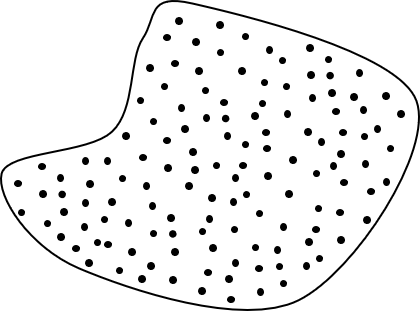
\includegraphics[scale=0.8]{./images/image11.png}
    \caption{连续体离散化成点云}
    \label{fig: discretise continuum}
\end{figure}

其次假设有限元函数空间为$$\{f: f(x) = \sum_\mathbf{i} f_\mathbf{i} B_\mathbf{i}(x), \mathbf{i} = ijk, i,j,k\in{1,2,3}\}$$因此
$\hat{v}^{n+1}(x) = \sum_{\mathbf{i}}\hat{v}^{n+1}_{\mathbf{i}}B_{\mathbf{i}}(x)$,$v^n(x) = \sum_{\mathbf{i}}v^n_{\textbf{i}}B_{\textbf{i}}(x)$,测试函数$w(x) = e_{\alpha}B_{\mathbf{i}}(x)$,这里$e_{\alpha}$为三维空间的第$\alpha\in\{1,2,3\}$个标准基。
带入(4.2)式左边有
\begin{align}
    \int_{\Omega^{t^n}}\rho(x,t^n)\frac{\hat{v}^{n+1}(x) - v^n(x)}{\Delta t}\cdot w dx &=  \int_{\Omega^{t^n}} \rho(x,t^n)\sum_{\mathbf{i}}\frac{\hat{v}^{n+1}_\mathbf{i} - v^n_{\mathbf{i}}}{\Delta t}B_\mathbf{i}(x)\cdot e_{\alpha}B_{\mathbf{j}}(x)dx\nonumber
\end{align}
右边为
\begin{align}
    \int_{\partial \Omega^{t^n}} (I - \tilde{n}\tilde{n}^T):e_{\alpha}\nabla B_{\mathbf{j}}(x) ds - \int_{\Omega^{t^n}}\lambda (det(F\circ \phi_t^{-1}) - 1)I:e_{\alpha}\nabla B_\mathbf{j}(x) dx
\end{align}
如果我们同时考虑$e_{\alpha},\alpha = 1,2,3$,这样上式即在三个维度统一表示为
\begin{align}
    \int_{\Omega^{t^n}}\rho(x,t^n)\sum_\mathbf{i} \frac{\hat{v}^{n+1}_\mathbf{i} - v^n_{\mathbf{i}}}{\Delta t}B_\mathbf{i}(x)B_\mathbf{j}(x)dx &= \int_{\partial \Omega^{t^n}} (I - \tilde{n}\tilde{n}^T)\nabla B_{\mathbf{i}}(x)^T ds \nonumber\\
                                                                            & - \int_{\Omega^{t^n}} \lambda (det(F\circ \phi_t^{-1}) - 1)\nabla B_\mathbf{i}(x)^T dx \nonumber     
\end{align}
对积分离散化我们有
\begin{align}
    \sum_\mathbf{i}\int_{\Omega^{t^n}}\rho(x,t^n) \frac{\hat{v}^{n+1}_\mathbf{i} - v^n_{\mathbf{i}}}{\Delta t}B_\mathbf{i}(x)B_\mathbf{j}(x)dx &\approx \sum_{\mathbf{i},p}B_\mathbf{i}(x_p^n)B_\mathbf{j}(x_p^n)\frac{\hat{v}^{n+1}_\mathbf{i} - v^n_{\mathbf{i}}}{\Delta t}\int_{\Omega^{t^n}_p}\rho(x,t)dx\nonumber\\
    &= \sum_{\mathbf{i},p}B_\mathbf{i}(x_p^n)B_\mathbf{j}(x_p^n)\frac{\hat{v}^{n+1}_\mathbf{i} - v^n_{\mathbf{i}}}{\Delta t}m_p
\end{align}
此处$p\in \mathcal{V}$为离散点云上的点,$x_p^n\in \mathbb{R}^3$为$t^n$时刻点$p$的位置,$m_p = \int_{\Omega_p^{t^n}} \rho(x,t)dx$,这里$m_p$为粒子$p$周围的质量,根据质量守恒,$m_p$与时间无关。
再记$\hat{M}_{\mathbf{j}\mathbf{i}} = \sum_p B_{\mathbf{j}}(x_p^n)B_{\mathbf{i}}(x_p^n)m_p$
通常我们会牺牲精度,使用矩阵行求和的方式~\cite{de2020material}来简化矩阵$\hat{M}$。即$M_{\mathbf{jj}} = \sum_{\mathbf{i}}\hat{M}_{\mathbf{ji}}$,$M$的非对角项为0。同时注意到,
B-样条的单位分解性,我们有
$$M_{\mathbf{jj}} = \sum_p m_p B_{\mathbf{j}}(x_p^n)\sum_\mathbf{i}B_\mathbf{i}(x_p^n) = \sum_p m_p B_{\mathbf{j}}(x_p^n)$$
同理我们可以得到
\begin{align}
    \int_{\Omega^{t^n}}\lambda (det(F\circ \phi_t^{-1}) - 1)\nabla B_{\mathbf{j}}(x)^Tdx &\approx \sum_p \lambda (det(F_p^n) - 1)\nabla B_{\mathbf{j}}(x_p^n)^T\int_{\Omega^{t^n}_p}dx \nonumber\\
    & = \sum_p \lambda (det(F_p^n) - 1)\nabla B_{\mathbf{j}}(x_p^n)^T V_p^n\nonumber \\
    & \approx \sum_p \lambda (det(F_p^n) - 1)\nabla B_{\mathbf{j}}(x_p^n)^T V_p^0\nonumber     
\end{align}
这里$F_p^n$为粒子$p$在$t^n$时刻的形变梯度,$V_p^n$为时刻$t^n$时$p$邻域小块$\Omega_p^{t^n}$的体积,由于我们将使用较大的体积惩罚来减小体积变化,因此我们可以近似$V_p^n$为初始时刻的体积$V_p^0$。

最后我们来处理表面积分项$\int_{\partial \Omega^{t^n}} (I - \tilde{n}\tilde{n}^T)\nabla B_{\mathbf{i}}(x)^T ds$,假定我们已经获取了点云在$t^n$时刻的表面,总表面积为$Area$,且已在表面上均匀的采点,每个点分配面积为$A_s = \frac{Area}{\#\mathcal{S}}$,表面点集为$\mathcal{S}$。
\begin{figure}[htbp]
    \centering
    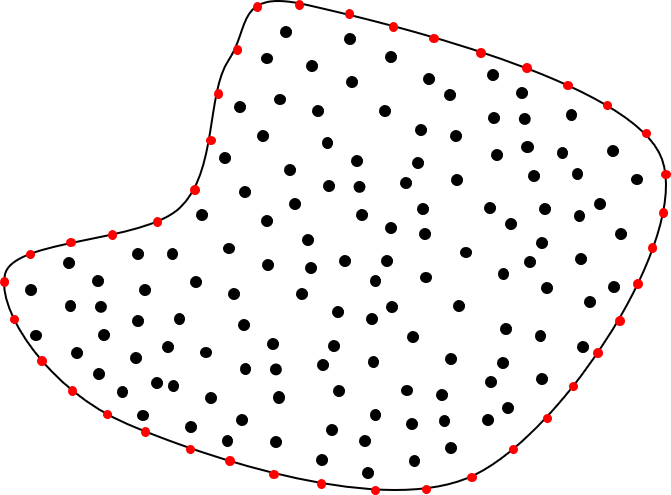
\includegraphics[scale=0.4]{./images/image12.png}
    \caption{红色点$s$为采样获得的表面点集$\mathcal{S}$}
    \label{fig: surface of point cloud}
\end{figure}

那么我们有
\begin{align}
    \int_{\partial \Omega^{t^n}} (I - \tilde{n}\tilde{n}^T)\nabla B_{\mathbf{j}}(x)^T ds &\approx \sum_{s\in\mathcal{S}}(I - \tilde{n}_s\tilde{n}_s^T)\nabla B_{\mathbf{j}}(x_s^n)^TA_s
\end{align}
将上述离散化结果整理我们得到
\begin{align}
    \sum_{p\in \mathcal{V}} \frac{\hat{v}^{n+1}_\mathbf{j} - v^n_{\mathbf{j}}}{\Delta t}m_pB_{\mathbf{j}}(x_p^n) = &k\sum_{s\in\mathcal{S}}(I - \tilde{n}_s\tilde{n}_s^T)\nabla B_{\mathbf{j}}(x_s^n)^TA_s\nonumber\\
    & - \lambda \sum_{p\in\mathcal{V}} (det(F_p^n) - 1)\nabla B_{\mathbf{j}}(x_p^n)^T V_p^0
\end{align}
如果记$m_{\mathbf{j}}^n = \sum_p m_p B_{\mathbf{j}}(x_p^n)$,则上述问题变为
\begin{align}
    m_\mathbf{j}^n \frac{\hat{v}^{n+1}_\mathbf{j} - v^n_{\mathbf{j}}}{\Delta t} &= k\sum_{s\in \mathcal{S}}(I - \tilde{n}_s\tilde{n}_s^T)\nabla B_\mathbf{j}(x_s^n)^TA_s\nonumber\\
    & - \lambda \sum_{p\in\mathcal{V}} (det(F_p^n) - 1)\nabla B_{\mathbf{j}}(x_p^n)^T 
\end{align}
自然我们给出$p$的位置$x_p^n$更新公式
\begin{align}    
    x_p^{n+1} = x_p^n + \Delta t \tilde{v}_p^{n+1}
\end{align}
同时回顾第二章的$\dot{F} = \nabla v \cdot F$,我们得到
\begin{align}
    F^{n+1}_p = (I + \Delta t\cdot \nabla {v}^{n+1}_p)F^n_p
\end{align}

\subsection{数据表示与储存}
从式(4.7),(4.8),(4.9)可以看到,我们需要的变量有$x_p^n\in \mathbb{R}^3,v_p^{n}\in \mathbb{R}^3,F_p^n\in \mathbb{R}^{3\times 3}$,这些变量我们都储存在粒子上,由于粒子上储存质量信息不会随着时间改变,因此该数据表示方式
自然的满足了质量守恒方程。如图\ref{fig: particle information}所示
\begin{figure}[htbp]
    \centering
    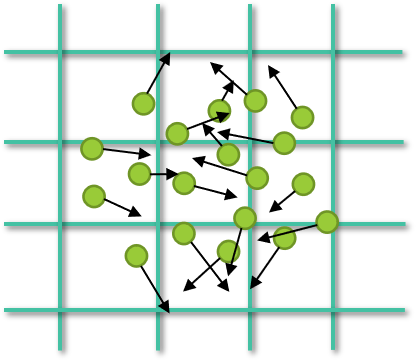
\includegraphics[scale=0.7]{./images/image13.png}
    \caption{粒子上的信息}
    \label{fig: particle information}
\end{figure}

同时注意到这里在$t^n$时刻需要参与计算的信息还有$v_\mathbf{j}^n \in \mathbb{R}^3$和$m_\mathbf{j}^n \in \mathbb{R}$,这里的信息我们储存在
格点上。如图\ref{fig: grid information}所示,这里我们注意到$m_{\mathbf{j}}^n = \sum_p m_p B_{\mathbf{j}}(x_p^n)$,此处实际上我们把粒子上的
数据分散到了网格上,同时注意到$\sum_{\mathbf{j}} m_\mathbf{j}^n = \sum_{\mathbf{j}}\sum_p m_p B_{\mathbf{j}}(x_p^n)$,这里再使用B-样条的单位分解性,我们有
$\sum_{\mathbf{j}}m_\mathbf{j} = \sum_p m_p$,因此该分配方式依然是质量守恒的过程。
\begin{figure}[htbp]
    \centering
    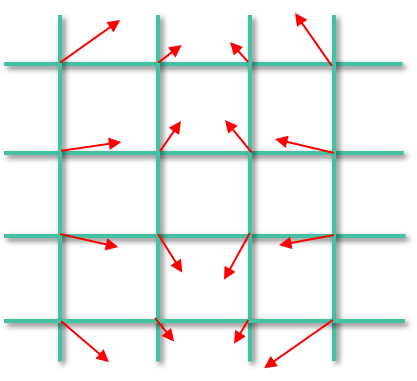
\includegraphics[scale=0.7]{./images/image14.png}
    \caption{格点上的信息}
    \label{fig: grid information}
\end{figure}

\section{数值修正}
在上一节得到连续方程的离散化之后,我们接下来给出该离散方程的计算策略以及一些工程实践上的修正。
\subsection{表面重建与粒子属性调整}
在给定的粒子集合$\mathcal{V}$以及$t^n$时刻每个粒子$p \in \mathcal{V}$的位置$x_p$时,我们可以使用第\ref{chap3}章
提到的方法重建表面网格,然后使用泊松圆盘采样获取表面的粒子$\mathcal{S}$。在构造隐式曲面时,我们需要额外的偏移量,此
处我们对每一个$s\in \mathcal{S}$,在$\mathcal{V}$中寻找距离$s$最近的粒子$p_s \in \mathcal{V}$,偏移方向
为$n_s = \frac{x_s - x_{p_s}}{\Vert x_s - x_{p_s} \Vert}$,如图\ref{fig: offset of surface particle}所示。我们将
$\mathcal{S}$和$\mathcal{N}$作为输入可以得到逼近的隐式曲面,然后估计$S$中表面粒子的法向$\tilde{n}_s$。
\begin{figure}[htbp]
    \centering
    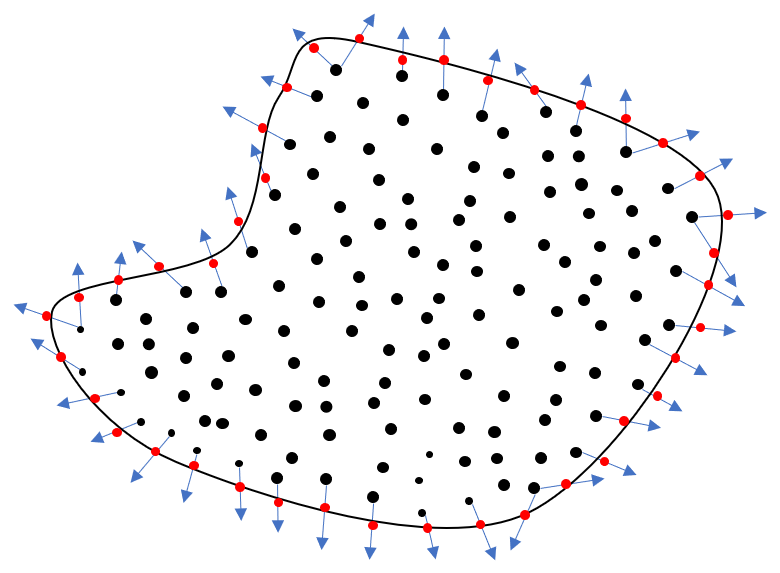
\includegraphics[scale=0.7]{./images/image15.png}
    \caption{箭头为偏移方向,红色点为表面粒子$s\in \mathcal{S}$,箭头起始端为$p_s \in\mathcal{V}$}
    \label{fig: offset of surface particle}
\end{figure}

在实践中,表面张力项$f^{surface} = k\sum_{s\in \mathcal{S}}(I - \tilde{n}_s\tilde{n}_s^T)\nabla B_{\mathbf{j}}(x_s^n)^TA_s$需要传导到内部粒子,与液体压力共同影响形变结果,如果表面粒子离内部粒子最短距离大于
$\sqrt{3}h$(即在$s$所占的一个格子之外),那么该表面粒子$s\in \mathcal{S}$将难以通过网格把表面张力传导到内部粒子。为了解决这一问题,我们对每一个表面粒子$s\in \mathcal{S}$寻找其在内部的最近的点$p_s \in \mathcal{V}$,
然后生成一个嵌入点$o_s$,嵌入点$o_s$的位置我们选取为$x_{o_s} = 2x_{p_s} - x_s$,嵌入点集合我们记为$\mathcal{O}$。显然,$\mathcal{O}$与$\mathcal{S}$有一一对应关系,而内部点$p\in\mathcal{V}$与表面点集可能是多对一,因此我们记录每一个内部点
$v$所相关的表面点个数$C_v$,同时我们将内部点的质量均匀的分布给表面粒子和嵌入粒子,即$m_s = m_{o_s} = \frac{m_{p_s}}{2C_{p_s} + 1}$,其中内部粒子$p_s$的质量$m_{p_s}$重新赋值为$m_s$。同样的,我们赋予当前时刻表面粒子速度$v_s^n = v_{p_s}^n$以及嵌入粒子$o_s$
的速度$v_{o_s}^n = v_{p_s}^n$。
\begin{figure}[htbp]
    \centering
    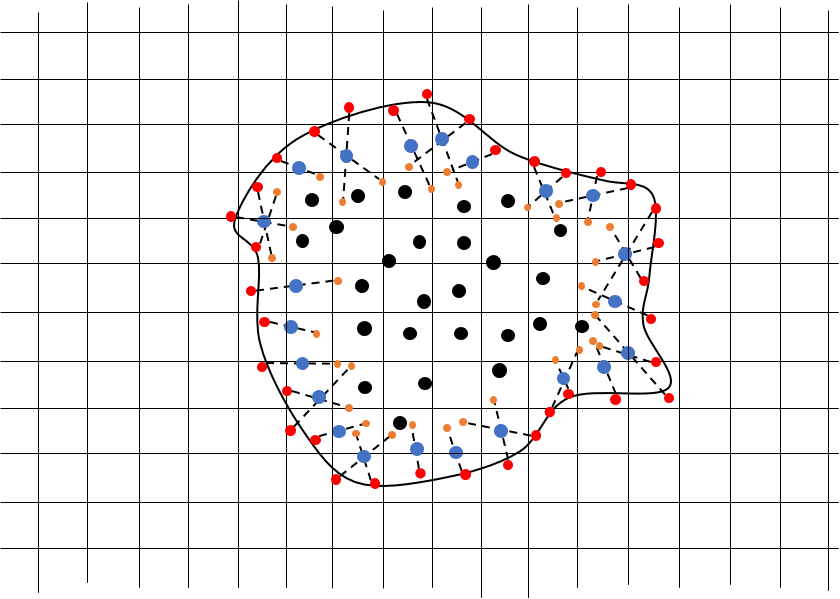
\includegraphics[scale=0.7]{./images/image16.png}
    \caption{红色点为表面粒子$s\in \mathcal{S}$,红色点通过虚线所连的蓝色点为离$s$最近的内部点$p_s\in \mathcal{V}$,橙色点$o_s\in \mathcal{O}$为新嵌入内部点}
    \label{fig: surface particle inserted}
\end{figure}
\subsection{粒子网格信息转换}
实际上在上一节中,我们已经给出了把粒子上的质量信息传递到网格上的计算公式,即$\tilde{m}^n_{\mathbf{j}} = \sum_p \tilde{m}_p B_{\mathbf{j}}(x_p^n)$。除了质量信息之外,我们仍然需要
速度信息$v_\mathbf{j}^n$,基于动量守恒的考虑~\cite{jiang2016material},我们采用的传递方式为将粒子的动量信息传递到网格上,再通过动量和质量的关系获取网格上的速度,即
\begin{align}
    (mv)_\mathbf{j}^n &= \sum_{p} \tilde{m}_p v_p^nB_{\mathbf{j}}(x_p^n)\\
    v_\mathbf{j}^n &= \frac{(mv)_\mathbf{j}^n}{m_{\mathbf{j}}^n} 
\end{align}
和质量守恒的证明方式类似,我们也可以证明该过程是动量守恒的,详细证明见~\cite{jiang2016material}。其中质量和动量的传递到网格过程我们称之为粒子转网格(Particle to Grid,简记为P2G)。

为了将网格速度信息转换到内部粒子(Grid to Particle,简记为G2P)上,最直观的办法是在粒子上采样空间网格上的速度场,即
\begin{align}
    v_p^n &= \sum_{\mathbf{i}} v_{\mathbf{i}}^n B_{\mathbf{i}}(x_p^n)
\end{align}
然而实际上,这样的采样办法只取得了速度的零阶信息,在实践中表现出来过粘的结果~\cite{tskhakaya2007particle},其中一种解决方案为保存空间速度场一阶速度信息,该方式被称为APIC~\cite{jiang2015affine}。
即对每个粒子额外添加$A_p^n \in \mathbb{R}^{3\times 3}$,一般而言$A_p^n$选取为速度场在$x_p^n$处的梯度,在APIC方法中选择为梯度的近似量。
\begin{align}
    A_p^n = \sum_{\mathbf{i}} \frac{4}{h^2}B_{\mathbf{i}}(x_p^n)v_{\mathbf{i}}^n(x_\mathbf{i} - x_p^n)^T
\end{align}
对于接近表面的内部粒子$\mathcal{V}_{\mathcal{S}} = \{p_s \in \mathcal{V}:p_s = \arg\min_{p \in \mathcal{V}} \Vert p - s\Vert, s\in \mathcal{S}\}$,
每一个$p\in \mathcal{V}_{\mathcal{S}}$记$\mathcal{N}_{p} = \{s\in \mathcal{S}:s = \arg\min_{s\in \mathcal{S}}\Vert p - s\Vert\}\cup \{o_s \in \mathcal{O}:s = \arg\min_{s\in \mathcal{S}}\Vert p - s\Vert\}$
为其相关的表面粒子集合。这里$p_s \in \mathcal{V}_\mathcal{S}$的近似梯度计算方式修正为
\begin{align}
    A_{p_s}^n = \frac{1}{2C_{p_s} + 1}\sum_{q \in \mathcal{N}_{p_s}\cup \{p_s\}}\sum_{\mathbf{i}} B_{\mathbf{i}}(x_q^n)\frac{4}{h^2}v_{\mathbf{i}}^n(x_\mathbf{i} - x_{p_s}^n)^T
\end{align}

在网格转粒子的步骤中添加了梯度信息的传递之后,我们修正P2G的过程。在每一个粒子上,我们使用仿射函数来近似粒子所携带的
速度$v_p^n(x) = v_p^n + A_p^n(x - x_p^n)$,这里动量传递据此修改为
\begin{align}
    (mv)_{\mathbf{j}}^n = \sum_{p}m_pv_p^n(x_\mathbf{j})B_{\mathbf{j}}(x_p^n)
\end{align}
同样的,表面粒子$s\in \mathcal{S}$与对应的嵌入粒子$o_s \in \mathcal{O}$也赋予
对应的梯度信息,$A_s = A_{o_s} = A_{p_s}$,这里$p_s$为$\mathcal{V}$中距离$s$最近的内部粒子,同样使用(4.15)式来传递到网格上。

在计算过程中,我们使用了$A_p^n$在近似替代$t^n$时刻速度场在位置$x_p^n$处的梯度,因此我们在更新形变梯度$F^n_p$时,为了节省计算量,我们也直接
将$\nabla v^n_p$替代为$A_p^n$,即
\begin{align}
    F_p^{n+1} = (I + A_p^{n+1})F_p^n
\end{align}
\subsection{网格上力的计算}
网格上由弱可压缩模型带来的力如下
\begin{align}
    f^{liquid}_{\mathbf{j}} = -\lambda \sum_p (det(F_p^n) - 1)\nabla B_{\mathbf{j}}^T(x_p^n)
\end{align}
由表面张力带来的效果为
\begin{align}
    f^{surface}_{\mathbf{j}} = k \sum_{s\in\mathcal{S}}(I - \tilde{n}_s\tilde{n}_s^T)\nabla B_{\mathbf{j}}(x_s^n)^TA_s
\end{align}
因此网格上的速度场更新为
\begin{align}
    \hat{v}_{\mathbf{j}}^{n+1} = \frac{1}{m_\mathbf{j}^n}(m_{\mathbf{j}}^nv_{\mathbf{j}}^n + \Delta t f^{liquid}_{\mathbf{j}} + \Delta t f^{surface}_{\mathbf{j}} +\Delta t m_\mathbb{j}^n g)
\end{align}
此处$g$为重力加速度。
\section{计算流程}
在前文给出了每一个步骤的计算细节之后,我们在本节总结算法的计算流程。首先我们的输入为粒子
集合$\mathcal{V}$及每个粒子$p\in\mathcal{V}$的预置位置$x_p^0$以及质量$m_p$。
默认初始化速度$v_p^0 = 0$,形变梯度与速度梯度为单位阵$I$。之后根据粒子的位置$x_p^n$激活相邻的空间网格,
并在激活网格上初始化$m_\mathbf{i}$与$v_\mathbf{i}$的内存,同时生成Marching cube所需的距离场。接下来,在激活的稀疏网格使用Marching Cube算法
提取距离场的水平集网格,并使用泊松圆盘采样在网格面上均匀采取表面粒子$\mathcal{S}$。然后我们估计表面粒子$s\in \mathcal{S}$的偏移量以及生成嵌入
粒子$\mathcal{O}$,该过程用到的临近粒子搜索依然可以利用稀疏网格$\mathcal{G}$做空间哈希。在有了偏移量之后,将偏移量和粒子位置作为输入,利用LSIPIA
拟合隐式曲面,并获得连续的法向。在这之后进行P2G,GOP,G2P三个步骤并更新粒子状态获得$x_p^{n+1},v_p^{n+1},F_p^{n+1},A_p^{n+1}$,并作为下一帧的输入。
同时我们输出当前时刻的$x_p^{n+1}$用作渲染。流程图见\ref{fig: pipline}。

\begin{figure}[htbp]
    \centering
    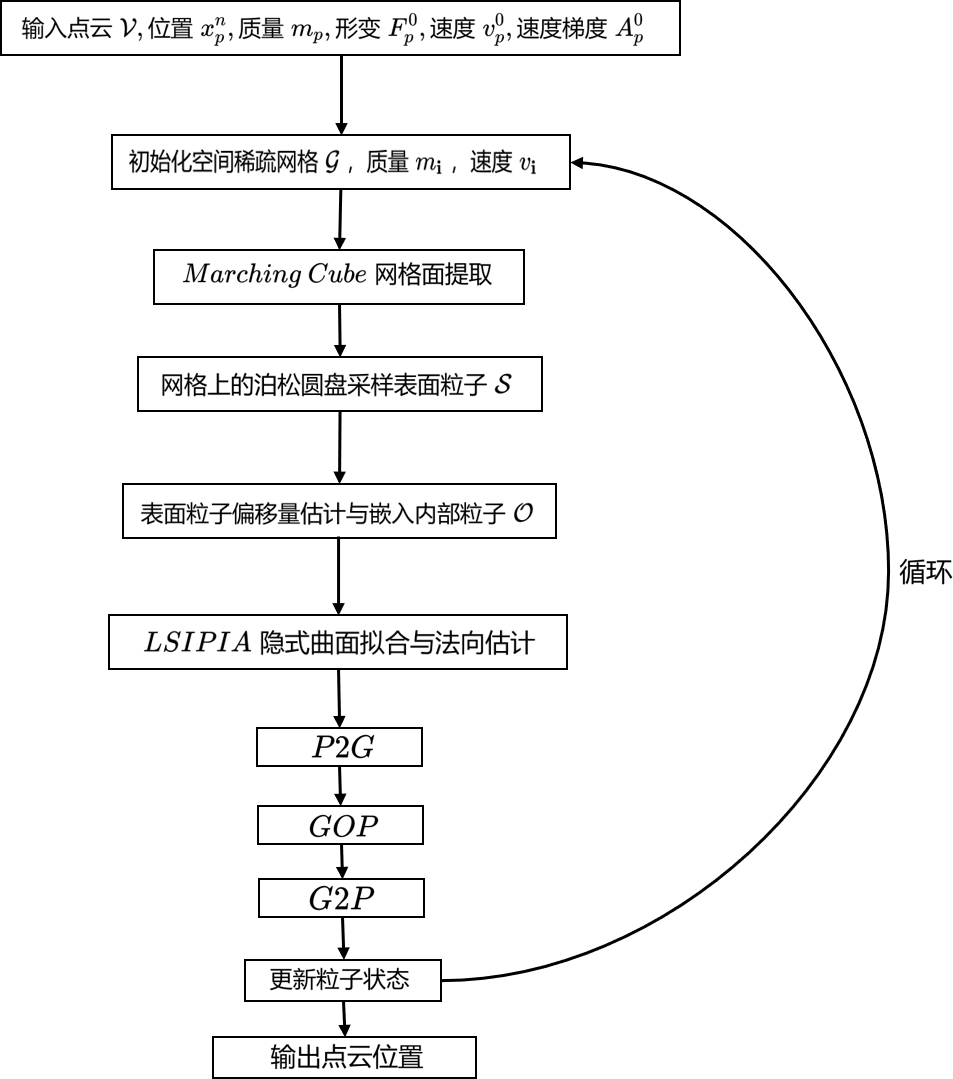
\includegraphics[scale=0.7]{./images/image17.png}
    \caption{计算流水线}
    \label{fig: pipline}
\end{figure}
\section{实验结果}

%literature
  \chapter{总结与展望}
\section{本文工作总结}
本文基于连续介质力学对流体表面张力与流体的抗压缩性进行建模,使用动量守恒以及本构模型给出了对应的偏微分方程。并且针对性的
对物质点法给出了表面张力的连续形式,并在伽辽金方法框架下将表面张力从边界条件转换到方程中,使其在物质点法的框架下易于离散。

同时本文利用了隐式曲面来拟合粒子表示的流体表面,相比于传统的网格方法可以更方便的实现拓扑变化。同时隐式曲面的拟合算法
大量复用了物质点法本身所需的数据结构,并通过改进迭代方式使其易于并行,相比原始的构建隐式曲面方法达到四个数量级的加速。
同样本文给出了一个配套的法向估计算法,在实践中与直接计算隐式曲面法向没有明显的差别,同时大大简化了计算流程,并让计算过程易于实现
单指令多数据流并行。

最后,本文将隐式曲面与物质点法的计算流程结合,给出了相应的偏微分方程离散化格式以及新的计算流程,并使用嵌入内部粒子的方式,
提高了辛积分格式在表面张力计算中的稳定性。为了验证本文给出的方法,我们给出了几个基本的数值实验,在几个测试集中本文方法成
功的捕捉到了流体表面张力以及抗压缩的特征并可以处理拓扑变化的情况。
\section{未来工作展望}
本文将表面张力融入了物质点法中,并针对物质点法改进表面重建的方法,使得其在速度和内存消耗上都有着很大的提升,但是该方法还有着很大的
改进空间以及进一步探索的空间。

1、进一步提高辛格式方法的稳定性,尽管本文能够求解一些例子,但是由于物质点法本身对时间步长要求较
严格,导致某些算例所需要的时间步长特别小,最终影响整体计算性能。

2、物质点法通过格点和粒子耦合,在长时间求解后会出现粒子聚集的问题,如何提高求解的长时间稳定性依然是需要解决的一个问题。

3、为了方便实现,本文对流体抗压缩性建模使用的为弱可压缩能量,最终在模拟上表现出一些不真实性。如何高效的将不可压缩限制条件
融入到求解流程,也是一个值得探索的方向。

4、物质点法本身在耦合多种物质求解取得了巨大的成功,在添加了表面张力之后,我们可以考虑添加流体更多的属性,
以及探索如何模拟流体和不同表面接触的效果。
%literature
%==============================================================
%这也是个不需要自己修改的部分。

  \backmatter %结束章节自动编号

%参考文献(习惯使用bibtex的可以修改)
  \addcontentsline{toc}{chapter}{参考文献} % 解决目录中没有相应的参考文献的条目问题
  \chaptermark{参考文献}
  
\begin{thebibliography}{200}
    \bibitem{article1} Ernest P . The philosophy of mathematics education by Paul Ernest[J]. Social Epistemology.

    \bibitem{article2} Bishop A J. Mathematical enculturation: a cultural perspective on mathematics education[J]. Journal for Research in Mathematics Education, 1988, 20(4):195.


\end{thebibliography}


%附录
  %  \include{chapters/appe}

% 出版物
  % \input{chapters/publication}

% 作者简历
  \chapter*{\centerline{作者简历}}
\chaptermark{作者简历}
\addcontentsline{toc}{chapter}{作者简历}


袁淳,男,1996年,汉族,江西龙南人。2015年考入上海金融学院(金融数学专业),2019年本科毕业,获得经济学学士学位。2019年进入浙江大学数学科学学院应用数学专业研究生学习至今。

% \begin{enumerate}
%     \item 工作经历
%     \begin{itemize}
%         \item 20XX-20XX年,在XX公司XX部门XX岗位
%         \item 20XX-20XX年,在XX公司XX部门XX岗位
%     \end{itemize}

%     \item 参与的项目
%     \begin{itemize}
%         \item 20XX-20XX年,参与XXXX项目
%         \item 20XX-20XX年,负责XXXX项目
%     \end{itemize}

%     \item 攻读学位期间发表的论文
%     \begin{itemize}
%         \item 猪八戒, 猪悟能, 天蓬元帅, 等. 论流体食物的持久保存[D]. 硕士学位论文. 北京: 广寒宫大学, 2005
%     \end{itemize}

% \end{enumerate}

%==============================================================
%==============================================================
\end{document}
